\ifdefined\maindoc\else
% typesetting this chapter as a standalone document
\def\doctitle{Finite Element Models}
% starting definitions for both the main document and stand-alone chapters
\documentclass{book}

\def\mech{artisynth.core.mechmodels}
\def\mgeo{maspack.geometry}

% Add search paths for input files
\makeatletter
\def\input@path{{../}{../../}{../texinputs/}}
\makeatother

\usepackage{amsmath}
\usepackage{framed}
%%
%% Default settings for artisynth
%%
\NeedsTeXFormat{LaTeX2e}
%%\ProvidesPackage{artisynthDoc}[2012/04/05]

\usepackage[T1]{fontenc}
\usepackage[latin1]{inputenc}
\usepackage{listings}
\usepackage{makeidx}
\usepackage{latexml}
\usepackage{graphicx}
\usepackage{framed}
\usepackage{booktabs}
\usepackage{color}

\newcommand{\pubdate}{\today}
\newcommand{\setpubdate}[1]{\renewcommand{\pubdate}{#1}}
\newcommand{\code}[1]{{\tt #1}}

\iflatexml
\usepackage{hyperref}
\setlength\parindent{0pt} 
\else
%% then we are making a PDF, so include things that LaTeXML can't handle: 
%% docbook style, \RaggedRight
\usepackage{ifxetex}
\usepackage{xstring}
\usepackage{pslatex} % fixes fonts; in particular sets a better-fitting \tt font

\usepackage[most]{tcolorbox}
\definecolor{shadecolor}{rgb}{0.95,0.95,0.95}
\tcbset{
    frame code={}
    center title,
    left=0pt,
    right=0pt,
    top=0pt,
    bottom=0pt,
    colback=shadecolor,
    colframe=white,
    width=\dimexpr\textwidth\relax,
    enlarge left by=0mm,
    boxsep=0pt,
    arc=0pt,outer arc=0pt,
}%

\usepackage[A4]{artisynth_papersize}
%\usepackage[letter]{artisynth_papersize}
\usepackage[hyperlink]{asciidoc-dblatex} 

%\usepackage{verbatim}
\usepackage{ragged2e}
\setlength{\RaggedRightRightskip}{0pt plus 4em}
\RaggedRight
\renewcommand{\DBKpubdate}{\pubdate}
\renewcommand{\DBKreleaseinfo}{}
\fi

% set hypertext links to be dark blue:
\definecolor{darkblue}{rgb}{0,0,0.8}
\definecolor{sidebar}{rgb}{0.5,0.5,0.7}
\hypersetup{colorlinks=true,urlcolor=darkblue,linkcolor=darkblue,breaklinks=true}

%%%%%%%%%%%%%%%%%%%%%%%%%%%%%%%%%%%%%%%%%%%%%%%%%%%%%%%%%%%%%%%%%%%%%%%%%%%%%
%
% Define macros for handling javadoc class and method references
%
%%%%%%%%%%%%%%%%%%%%%%%%%%%%%%%%%%%%%%%%%%%%%%%%%%%%%%%%%%%%%%%%%%%%%%%%%%%%%
\makeatletter

% macro to enable line break if inside a PDF file
\def\pdfbreak{\iflatexml\else\\\fi}

% code inspired by http://stackoverflow.com/questions/2457780/latex-apply-an-operation-to-every-character-in-a-string
\def\removeargs #1{\doremoveargs#1$\wholeString\unskip}
\def\doremoveargs#1#2\wholeString{\if#1$%
\else\if#1({()}\else{#1}\taketherest#2\fi\fi}
\def\taketherest#1\fi
{\fi \doremoveargs#1\wholeString}

% Note: still doesn't work properly when called on macro output ...
% i.e., \dottoslash{\concatnames{model}{base}{foo}} fails 
\def\dottoslash #1{\dodottoslash#1$\wholeString\unskip}
\def\dodottoslash#1#2\wholeString{\if#1$%
\else\if#1.{/}\else{#1}\fi\dottaketherest#2\fi}
\def\dottaketherest#1\fi{\fi \dodottoslash#1\wholeString}

\def\hashtodot #1{\dohashtodot#1$\wholeString\unskip}
\def\dohashtodot#1#2\wholeString{\if#1$X%
\else\if#1\#{.}\else{#1}\fi\hashtaketherest#2\fi}
\def\hashtaketherest#1\fi{\fi \dohashtodot#1\wholeString}

%\dollartodot{#1} does the same thing as \StrSubstitute[0]{#1}{\$}{.}
% from the packahe xstring. We define \dollartodot instead because
% LaTeXML does not implement xstring.
%
% Note that for the substituion to work, we need \ifx instead of \if,
% since otherwise escaped characters won't work properly:
% if #1 = \$, then \if#1* seems to compare '\' and '$' (and output '*'),
% rather than comparing '$' to '*'
\def\dollartodot #1{\dodollartodot#1*\wholeString\unskip}
\def\dodollartodot#1#2\wholeString{\ifx#1*%
\else \ifx#1\${.}\else{#1}\fi\dollartaketherest#2\fi}
\def\dollartaketherest#1\fi{\fi \dodollartodot#1\wholeString}

% concatenates up to three class/method names together, adding '.' characters
% between them. The first and/or second argument may be empty, in which case
% the '.' is omitted. To check to see if these arguments are empty, we
% use a contruction '\if#1@@', which will return true iff #1 is empty
% (on the assumption that #1 will not contain a '@' character).
\def\concatnames
#1#2#3{\if#1@@\if#2@@#3\else #2.#3\fi\else\if#2@@#1.#3\else#1.#2.#3\fi\fi}

\newcommand{\javabase}{}
\newcommand{\setjavabase}[1]{\renewcommand{\javabase}{#1}}

\def\artisynthDocBase{@ARTISYNTHDOCBASE}

\iflatexml
\def\ifempty#1{\def\temp{#1}\ifx\temp\empty}%
\newcommand{\artisynthManual}[3][]{%
   \ifempty{#1}
      \href{@ARTISYNTHDOCBASE/#2/#2.html}{#3}%
    \else
      \href{@ARTISYNTHDOCBASE/#1/#2.html}{#3}%
    \fi
}
\else
\newcommand{\artisynthManual}[3][]{%
\href{https://www.artisynth.org/@ARTISYNTHDOCBASE/#2.pdf}{#3}}
\fi

%\href{@ARTISYNTHDOCBASE/#2/#2.html}{#3}}



\newcommand{\javaclassx}[2][]{%
% Includes code to prevent an extra '.' at the front if #1 is empty. It
% works like this: if '#1' is empty, then '#1.' expands to '.', and so 
% '\if#1..' will return true, in which case we just output '#2'.
\href{@JDOCBEGIN/\concatnames{\javabase}{#1}{#2}@JDOCEND}{#2}}
\newcommand{\javaclass}[2][]{%
\href{@JDOCBEGIN/\concatnames{}{#1}{#2}@JDOCEND}{\dollartodot{#2}}}
\newcommand{\javaclassAlt}[2]{%
\href{@JDOCBEGIN/\concatnames{}{}{#1}@JDOCEND}{#2}}

\newcommand{\javamethodArgsx}[2][]{%
\href{@JDOCBEGIN/\concatnames{\javabase}{#1}{#2}@JDOCEND}{#2}}
\newcommand{\javamethodArgs}[2][]{%
\href{@JDOCBEGIN/\concatnames{}{#1}{#2}@JDOCEND}{#2}}
\newcommand{\javamethodAlt}[2]{%
\href{@JDOCBEGIN/\concatnames{}{}{#1}@JDOCEND}{#2}}
\newcommand{\javamethodAltx}[2]{%
\href{@JDOCBEGIN/\concatnames{\javabase}{}{#1}@JDOCEND}{#2}}

\newcommand{\javamethodNoArgsx}[2][]{%
\href{@JDOCBEGIN/\concatnames{\javabase}{#1}{#2}@JDOCEND}{\removeargs{#2}}}
\newcommand{\javamethodNoArgs}[2][]{%
\href{@JDOCBEGIN/\concatnames{}{#1}{#2}@JDOCEND}{\removeargs{#2}}}

\newcommand{\javamethod}{\@ifstar\javamethodNoArgs\javamethodArgs}
\newcommand{\javamethodx}{\@ifstar\javamethodNoArgsx\javamethodArgsx}

%%%%%%%%%%%%%%%%%%%%%%%%%%%%%%%%%%%%%%%%%%%%%%%%%%%%%%%%%%%%%%%%%%%%%%%%%%%%%
%
% Define macros for sidebars
%
%%%%%%%%%%%%%%%%%%%%%%%%%%%%%%%%%%%%%%%%%%%%%%%%%%%%%%%%%%%%%%%%%%%%%%%%%%%%%

\iflatexml
\newenvironment{sideblock}{\begin{quote}}{\end{quote}}
\else
\usepackage[strict]{changepage}
\definecolor{sidebarshade}{rgb}{1.0,0.97,0.8}
\newenvironment{sideblock}{%
    \def\FrameCommand{%
    \hspace{1pt}%
    {\color{sidebar}\vrule width 2pt}%
    %{\vrule width 2pt}%
    {\color{sidebarshade}\vrule width 4pt}%
    \colorbox{sidebarshade}%
  }%
  \MakeFramed{\advance\hsize-\width\FrameRestore}%
  \noindent\hspace{-4.55pt}% disable indenting first paragraph
  \begin{adjustwidth}{}{7pt}%
  %\vspace{2pt}\vspace{2pt}%
}
{%
  \vspace{2pt}\end{adjustwidth}\endMakeFramed%
}
\fi

\iflatexml
\newenvironment{shadedregion}{%
  \definecolor{shadecolor}{rgb}{0.96,0.96,0.98}%
  \begin{shaded*}%
% Put text inside a quote to create a surrounding blockquote that
% will properly accept the color and padding attributes
  \begin{quote}%
}
{%
  \end{quote}%
  \end{shaded*}%
}
\else
\newenvironment{shadedregion}{%
  \definecolor{shadecolor}{rgb}{0.96,0.96,0.98}%
  \begin{shaded*}%
}
{%
  \end{shaded*}%
}
\fi

% Wanted to create a 'listing' environment because lstlisting is
% tedious to type and because under latexml it may need
% some massaging to get it to work properly. But hard to do
% because of the verbatim nature of listing
%\iflatexml
%\newenvironment{listing}{\begin{lstlisting}}{\end{lstlisting}}%
%\else
%\newenvironment{listing}{\begin{lstlisting}}{\end{lstlisting}}%
%\fi

\iflatexml\else
% fancyhdr was complaining that it wanted a 36pt header height ...
\setlength{\headheight}{36pt}
\fi

% macro for backslash character
\newcommand\BKS{\textbackslash}

% macro for double hyphen (to prevent conversion of -- into -)
\newcommand\DHY{-{}-}

% Convenience stuff
\newcommand{\ifLaTeXMLelse}[2]{%
  \iflatexml %
  #1 %
  \else %
  #2 %
  \fi %
}

\newcommand{\ifLaTeXML}[1]{ %
  \iflatexml %
  #1 %
  \fi %
}

% new methodtable environment for documenting methods

% base width of the method table
\newlength{\methodtablewidth}
\iflatexml
\setlength{\methodtablewidth}{1.4\textwidth}
\else
\setlength{\methodtablewidth}{0.94\textwidth}
\fi
% horizontal space added at end of call to \methodentry
\newlength{\methodskip}
\setlength{\methodskip}{0pt}
% lengths set inside methodtable environment:
\newlength{\methodsiglength} % length of the method signature
\newlength{\methodcomlength} % length of the method comment
\setlength{\methodsiglength}{0.5\methodtablewidth}
\setlength{\methodcomlength}{0.5\methodtablewidth}

% command to add a method to a method table:
% arg #1: package and signature for finding URL
% arg #2: anchor text
% arg #3: comment describing the method
\newcommand{\methodentry}[3]{%
\javamethodAlt{#1}{\parbox[t]{\methodsiglength}{#2}}&
{\parbox[t]{\methodcomlength}{#3}}\\%
\noalign{\vspace{\methodskip}}}

% methodtable environment takes two arguments, both scale factors for
% methodtablewidth:
% arg #1: width of the method signature column
% arg #2: width of the method comment column
\newenvironment{methodtable}[3][0pt]{%
\begingroup
\setlength{\topskip}{0pt}
\setlength{\methodskip}{#1}
\setlength{\methodsiglength}{#2\methodtablewidth}%
\setlength{\methodcomlength}{#3\methodtablewidth}%
\iflatexml
\begin{snugshade}
\else
\begin{tcolorbox}
\fi
\renewcommand{\arraystretch}{1}
\begin{tabular}{ll}}{%
\end{tabular}
\renewcommand{\arraystretch}{1}
\iflatexml
\end{snugshade}
\else
\end{tcolorbox}
\fi
\endgroup}

% commands for added top, mid and bottom lines in the table.
% uses booktabs for PDF, regular hline for HTML
\newcommand{\topline}{\iflatexml\hline\else\toprule\fi}
\newcommand{\midline}{\iflatexml\hline\else\midrule\fi}
\newcommand{\botline}{\iflatexml\hline\else\bottomrule\fi}
\newcommand{\blankline}{%
\multicolumn{2}{l}{\iflatexml{@SPACE}\else\phantom{M}\fi}\\}%
% add vertical space within a two colum method environment
\newcommand{\methodspace}[1]{%
\iflatexml
\multicolumn{2}{l}{@VERTSPACE[#1]}\\
\else
\noalign{\vspace{#1}}%
\fi}%
% break a line and add an indentation of 1em
\newcommand{\brh}{\\\phantom{M}}

\makeatother

\def\matl{\left(\begin{matrix}}
\def\matr{\end{matrix}\right)}

\def\Bthe{\boldsymbol\theta}
\def\Btau{\boldsymbol\tau}
\def\Bom{\boldsymbol\omega}
\def\Bdel{\boldsymbol\delta}
\def\Blam{\boldsymbol\lambda}
\def\Bphi{\boldsymbol\phi}
\def\Bxi{\boldsymbol\xi}
\def\Bgam{\boldsymbol\gamma}
\def\Bsig{\boldsymbol\sigma}
\def\Bnu{\boldsymbol\nu}
\def\Bmu{\boldsymbol\mu}

\def\A{{\bf A}}
\def\B{{\bf B}}
\def\C{{\bf C}}
\def\D{{\bf D}}
\def\F{{\bf F}}
\def\G{{\bf G}}
\def\H{{\bf H}}
\def\I{{\bf I}}
\def\J{{\bf J}}
\def\K{{\bf K}}
\def\Jc{{\bf J}_c}
\def\L{{\bf L}}
\def\M{{\bf M}}
\def\N{{\bf N}}
\def\O{{\bf O}}
\def\P{{\bf P}}
\def\Q{{\bf Q}}
\def\R{{\bf R}}
\def\T{{\bf T}}
\def\U{{\bf U}}
\def\W{{\bf W}}
\def\X{{\bf X}}
\def\Minv{{\bf M}^{-1}}

\def\a{{\bf a}}
\def\b{{\bf b}}
\def\c{{\bf c}}
\def\d{{\bf d}}
\def\e{{\bf e}}
\def\f{{\bf f}}
\def\g{{\bf g}}
\def\k{{\bf k}}
\def\l{{\bf l}}
\def\m{{\bf m}}
\def\n{{\bf n}}
\def\p{{\bf p}}
\def\q{{\bf q}}
\def\r{{\bf r}}
\def\u{{\bf u}}
\def\v{{\bf v}}
\def\w{{\bf w}}
\def\x{{\bf x}}
\def\y{{\bf y}}
\def\z{{\bf z}}

\def\ma{{\bf m}_\alpha}
\def\mb{{\bf m}_\beta}
\def\va{{\bf v}_\alpha}
\def\vb{{\bf v}_\beta}
\def\vp{{\bf v}_\rho}
\def\vk{{\bf v}_k}
\def\ua{{\bf u}_\alpha}
\def\ub{{\bf u}_\beta}
\def\uk{{\bf u}_k}
\def\uj{{\bf u}_j}
\def\mar{{\bf m}_{\alpha r}}
\def\mbr{{\bf m}_{\beta r}}

\def\Maa{{\bf M}_{\alpha\alpha}}
\def\Mab{{\bf M}_{\alpha\beta}}
\def\Mba{{\bf M}_{\beta\alpha}}
\def\Mbb{{\bf M}_{\beta\beta}}
\def\hatMaa{\hat{\bf M}_{\alpha\alpha}}
\def\hatMab{\hat{\bf M}_{\alpha\beta}}
\def\hatMba{\hat{\bf M}_{\beta\alpha}}
\def\hatMbb{\hat{\bf M}_{\beta\beta}}
\def\Mbp{{\bf M}_{\beta\rho}}
\def\Map{{\bf M}_{\alpha\rho}}
\def\Mpa{{\bf M}_{\rho\alpha}}
\def\Mpb{{\bf M}_{\rho\beta}}
\def\Mpp{{\bf M}_{\rho\rho}}
\def\Mbk{{\bf M}_{\beta k}}
\def\Mak{{\bf M}_{\alpha k}}
\def\Mka{{\bf M}_{k\alpha}}
\def\Mkb{{\bf M}_{k\beta}}
\def\Mkk{{\bf M}_{kk}}

\def\Ga{{\bf G}_{\alpha}}
\def\Gp{{\bf G}_{\rho}}
\def\Gaa{{\bf G}_{\alpha\alpha}}
\def\Gab{{\bf G}_{\alpha\beta}}
\def\Gba{{\bf G}_{\beta\alpha}}
\def\Gbb{{\bf G}_{\beta\beta}}
\def\Gap{{\bf G}_{\alpha\rho}}
\def\Gpa{{\bf G}_{\rho\alpha}}
\def\Gbp{{\bf G}_{\beta\rho}}
\def\Gak{{\bf G}_{\alpha k}}
\def\Gka{{\bf G}_{k\alpha}}
\def\Gja{{\bf G}_{j\alpha}}
\def\Gkb{{\bf G}_{k\beta}}
\def\Gbk{{\bf G}_{\beta k}}

\def\lama{\Blam_{\alpha}}
\def\lamb{\Blam_{\beta}}
\def\lamp{\Blam_{\rho}}
\def\lamk{\Blam_{k}}
\def\lams{\Blam_{\sigma}}

\def\ba{{\bf b}_{\alpha}}
\def\bb{{\bf b}_{\beta}}
\def\fp{{\bf f}_{\rho}}
\def\fa{{\bf f}_{\alpha}}
\def\qa{{\bf q}_{\alpha}}
\def\qb{{\bf q}_{\beta}}
\def\za{{\bf z}_{\alpha}}
\def\zb{{\bf z}_{\beta}}
\def\wa{{\bf w}_{\alpha}}
\def\wb{{\bf w}_{\beta}}

\def\Na{\bar{\bf N}_{\alpha}}
\def\Nb{\bar{\bf N}_{\beta}}

\def\Up{{\bf U}_p}
\def\Un{{\bf U}_n}

\def\dFdl{\frac{\partial F}{\partial l}}
\def\dFddl{\frac{\partial F}{\partial \dot l}}

\def\Sr{s_\theta}
\def\Cr{c_\theta}
\def\Sp{s_\phi}
\def\Cp{c_\phi}
\def\Sy{s_\psi}
\def\Cy{c_\psi}
\def\Sa{s_{\alpha}}
\def\Ca{c_{\alpha}}
\def\Vp{v_{\phi}}


\iflatexml
\else
\usepackage{biblatex}
\addbibresource{references.bib}
\fi

\setcounter{tocdepth}{5}
\setcounter{secnumdepth}{3}

\title{\doctitle}
\ifdefined\maindoc
\author{John Lloyd and Antonio S\'anchez}
\setpubdate{Last update: March, 2022}

\iflatexml
\date{}
\fi
\fi

% graphics paths
\graphicspath{{./}{images/}}

% Listings settings
\definecolor{myblue}{rgb}{0,0,0.6}
\definecolor{mygreen}{rgb}{0,0.6,0}
\definecolor{mygray}{rgb}{0.5,0.5,0.5}
\definecolor{mylightgray}{rgb}{0.95,0.95,0.95}
\definecolor{mymauve}{rgb}{0.58,0,0.82}
\definecolor{myblack}{rgb}{0,0,0}
\lstset{
   language=Java,                   % text highlighting for Java
   breakatwhitespace=false,         % automatic breaks only at whitespace
   breaklines=true,                 % automatic line breaking
   commentstyle=\color{mygreen},    % comment style
   keepspaces=true,                 % keeps spaces in text
   keywordstyle=\color{myblue},     % keyword style
   numbers=none,                    % line-numbers; values: (none, left, right)
   numbersep=5pt,                   % how far the line-numbers are from code
   numberstyle=\tiny\color{mygray}, % line-numbers style
   showspaces=false,                % show spaces everywhere
   showstringspaces=false,          % underline spaces within strings
   showtabs=false,                  % show tabs
   stepnumber=1,                    % the step between two line-numbers
   stringstyle=\color{mymauve},     % string literal style
   tabsize=3,                       % sets default tabsize to 3 spaces
   backgroundcolor=\color{mylightgray}, % background color
   frame=single, 					% adds a frame around the code
   rulesepcolor=\color{mygray},
   rulecolor=\color{myblack},
   framerule=0pt,
   xleftmargin=2.2ex,               % numbers inside box
   framexleftmargin=2.2ex,			% indentation of frame
}

\begin{document}

\frontmatter

%\layout
\maketitle

\iflatexml{\large\pubdate}\fi

\tableofcontents

\mainmatter
\fi

% Scale latexml image sizes 2x
\newlength{\imglength}
\newcommand{\setlengthLaTeXML}[3]{ %
 \iflatexml %
 \setlength{#1}{#2} %
 \else %
 \setlength{#1}{#3} %
 \fi %
}

\chapter{Finite Element Models}
\label{FEMModels:sec}

This chapter details how to construct three-dimensional finite element models,
and how to couple them with the other simulation components described in
previous sections (e.g.~particles and rigid bodies).  Finite element
\emph{muscles}, which have additional properties that allow them to contract
given activation signals, are discussed in Section \ref{sec:fem:muscle}.  An 
example FEM model of the masseter, coupled to a rigid jaw and maxilla, is shown 
in Figure \ref{fig:fem:masseter}.

\begin{figure}[ht]
\centering
\setlengthLaTeXML{\imglength}{0.8\textwidth}{0.6\textwidth}
\includegraphics[width=\imglength]{images/fem_masseter}
\caption{Finite element model of the masseter, coupled to the jaw and 
maxilla. \label{fig:fem:masseter}} 
\end{figure}

\section{Overview}
\label{sec:fem:overview}

The finite element method (FEM) is a numerical technique used for solving a 
system of partial differential equations (PDEs) over some domain.  The general
approach is to divide the domain into a set of building blocks, referred to
as \emph{elements}.  These partition the space, and form local domains over
which the system of equations can be locally approximated. The corners of these
elements, the \emph{nodes}, become control points in a discretized system.  
The solution is then assumed to be
smoothly interpolated across the elements based on values determined at the
nodes.  Using this discretization, the differential system is converted into 
an algebraic one, which is often linearized and solved iteratively.

In ArtiSynth, the PDEs considered are the governing equations of
continuum mechanics: the conservation of mass, momentum, and energy.  To 
complete the system, a \emph{constitutive equation} is required that describes
the stress-strain response of the material.  This constitutive equation is what
distinguishes between material types.  The domain is the three-dimensional space
that the model occupies. This must be divided into small elements which 
accurately represent the geometry. Within each element, the PDEs are
sampled at a set of points, referred to as \emph{integration points}, and 
terms are numerically integrated to form an algebraic system to solve.

The purpose of the rest of this chapter is to describe the construction and
use of finite elements models within ArtiSynth.  It does not further discuss 
the mathematical framework or theory.
For an in-depth coverage of the nonlinear finite element method, as applied
to continuum mechanics, the reader is referred to the textbook by Bonet and 
Wood \cite{bonet:fem:2000}.

\subsection{FemModel3d}
\label{sec:fem:structure}

The basic type of finite element model is implemented in the class 
\javaclass[artisynth.core.femmodels]{FemModel3d}.  This class controls some
properties that are used by the model as a whole.  The key ones that affect
simulation dynamics are:
\begin{center}
\begin{tabular}{|ll|}
\hline
Property & Description\\
\hline
{\tt density} & The density of the model\\
{\tt material} & An object that describes the material's 
\emph{constitutive law} (i.e.~its stress-strain relationship).\\
{\tt particleDamping} & Proportional damping associated with the 
particle-like motion of the FEM nodes.\\
{\tt stiffnessDamping} & Proportional damping associated with the 
system's stiffness term.\\
\hline
\end{tabular}
\end{center}
These properties can be set and retrieved using the methods
\begin{lstlisting}[]
    setDensity (double density);    // sets the density
    double getDensity ();           // gets the density

    setMaterial (FemMaterial mat);  // sets the FEM's material
    FemMaterial getMaterial ();     // gets the FEM's material

    setParticleDamping (double d);  // sets the particle (mass) damping coefficient
    double getParticleDamping ();   // gets the particle (mass) damping coefficient

    setStiffnessDamping (double d); // sets the stiffness damping coefficient
    double getStiffnessDamping ();  // gets the stiffness damping coefficient
\end{lstlisting}
Keep in mind that ArtiSynth is essentially ``unitless'' (Section 
\ref{sec:mechii:units}), so it is the responsibility of the developer to
ensure that all properties are specified in a compatible way.  

The density of the model is used to compute the mass distribution
throughout the volume.  Note that we use a \emph{diagonally lumped
mass matrix} (DLMM) formulation, so the mass is assumed to be
concentrated at the location of the discretized FEM nodes.  To allow
for a spatially-varying density, densities can be explicitly set for
individual elements, or masses can be explicitly set for individual
nodes.

The FEM's {\sf material} property is a delegate object used to compute
stress and stiffness within individual elements.  It handles
the \emph{constitutive} component of the model, as described in more
detail in Section \ref{sec:fem:materials}.
In addition to the main material defined
for the model, it is also possible set a material on a per-element
basis, and to define additional materials which augment the behavior
of the main materials (Section \ref{sec:augmentingMaterials}).

The two damping parameters are related to \emph{Rayleigh damping}, which
is used to dissipate energy within finite element models.  There are two 
proportional damping terms: one related to the system's mass, and one related 
to stiffness.  The resulting damping force applied is
\begin{align}
	\f_d & = - (d_M \M + d_K\K)\v,
\end{align}
where $d_M$ is the value of {\tt particleDamping}, $d_K$ is the value of 
{\tt stiffnessDamping}, $\M$ is the FEM model's lumped mass matrix, $\K$ is 
the FEM's stiffness matrix, and $\v$ is the concatenated vector of FEM node
velocities.  Since the lumped mass matrix is diagonal, the mass-related
component of damping can be applied separately to each FEM node.  Thus, the
mass component reduces to the same system as Equation \eqref{eqn:pointdamping},
which is why it is referred to as ``particle damping''.

\subsection{Component Structure}
\label{sec:componentStructure}

Each \javaclass[artisynth.core.femmodels]{FemModel3d} contains several 
lists of sub-components:

\begin{description}
\item[{\tt nodes}]\mbox{}

The particle-like dynamic components of the model.  These lie at the corners
of the elements and carry all the mass (due to DLMM formulation).

\item[{\tt elements}]\mbox{}

The volumetric model elements. These define the 3D 
sub-units over which the system is numerically integrated.

\item[{\tt shellElements}]\mbox{}

The shell elements. These define additional 2D sub-units
over which the system is numerically integrated.

\item[{\tt meshes}]\mbox{}

The geometry in the model.  This includes the surface mesh, and any other
embedded geometries.

\item[{\tt materials}]\mbox{}

Optional additional materials which can be added to the
model to augment the behavior of the 
model's {\sf material} property. This is described in more detail
in Section \ref{sec:augmentingMaterials}.

\item[{\tt fields}]\mbox{}

Optional {\it field} components which can be used to interpolate
application-defined quantities over the FEM model's domain. Fields are
described in detail in Section \ref{sec:fields}.

\end{description}

The {\tt nodes}, {\tt elements} and {\tt meshes} components are
illustrated in Figure \ref{fig:fem}.

\begin{figure}[ht]
\centering
\setlengthLaTeXML{\imglength}{1.5in}{1.2in}
\begin{tabular}{cccc}
\includegraphics[width=\imglength]{images/fem_embedded} & 
\includegraphics[width=\imglength]{images/fem_embedded_nodes} &
\includegraphics[width=\imglength]{images/fem_embedded_elements} &
\includegraphics[width=\imglength]{images/fem_embedded_geometry}\\
(a) FEM model & (b) Nodes & (c) Elements & (d) Geometry
\end{tabular}
\caption{
Sub-components of \javaclass[artisynth.core.femmodels]{FemModel3d}. 
\label{fig:fem}}
\end{figure}

\subsubsection{Nodes}
\ifLaTeXML{\newline}

The set of nodes belong to a finite element model can be obtained by the method
\begin{lstlisting}[]
PointList<FemNode3d> getNodes();  // returns list of FEM nodes
\end{lstlisting}
Nodes are implemented in the class 
\javaclass[artisynth.core.femmodels]{FemNode3d}, which is a subclass of 
\javaclass[artisynth.core.mechmodels]{Particle} (Section 
\ref{ParticlesAndSprings:sec}).  They are the main dynamic components of
the finite element model.  The key properties affecting simulation dynamics
are:
\begin{center}
\begin{tabular}{|ll|}
  \hline
  Property & Description\\
  \hline
  {\tt restPosition} & The initial position of the node.\\
  {\tt position} & The current position of the node.\\
  {\tt velocity} & The current velocity of the node.\\
  {\tt mass} & The mass of the node.\\
  {\tt dynamic} & Whether the node is considered dynamic or parametric 
                  (e.g.~boundary condition).\\
  \hline
\end{tabular}
\end{center}
Each of these properties has corresponding {\tt getXxx()} and 
{\tt setXxx(...)} functions to access and modify them.

The {\tt restPosition} property defines the node's position in the FEM model's 
``natural'' or ``undeformed'' state.  Rest positions are used to compute
an initial configuration for the model, from which strains are determined.  A
node's rest position can be updated in code using the method:
\javamethod[artisynth.core.femmodels]{FemNode3d.setRestPosition(Point3d)}.

\begin{sideblock}
If any node's rest positions are changed, the current values 
for stress and stiffness will become invalid.  They can be manually
updated using the method \javamethod[artisynth.core.femmodels] %
{FemModel3d.updateStressAndStiffness()} for the parent model. Otherwise,
stress and stiffness will be automatically updated at the beginning of the 
next time step. 
\end{sideblock}

The properties {\tt position} and {\tt velocity} give the node's current
3D state.  These are common to all point-like particles, as is the 
{\tt mass} property.  Here, however, {\tt mass} represents the lumped mass
of the immediately surrounding material.  Its value is initialized by equally
dividing mass contributions from each adjacent element, given their
densities.  For a finer control of spatially-varying density,
node masses can be set manually after FEM creation.

The FEM node's {\tt dynamic} property specifies whether or not the 
node is considered when computing the dynamics of the system.  If not,
it is treated as being parametrically controlled.  This has implications
when setting boundary conditions (Section \ref{sec:fem:boundary}).

\subsubsection{Elements}
\ifLaTeXML{\newline}

Elements are the 3D volumetric spatial building blocks of the domain.
Within each element, the displacement (or strain) field is
interpolated from displacements at nodes:
\begin{align}
	\u(\x) & = \sum_{i=1}^N \phi_i(\x)\u_i, \label{eqn:fem:interp}
\end{align}
where $\u_i$ is the displacement of the $i$th node that is adjacent to the 
element, and $\phi_i(\cdot)$ is referred to as the \emph{shape function} (or 
\emph{basis function}) associated with that node.  Elements are classified by 
their shape, number of nodes, and shape function order (Table 
\ref{tbl:fem:elements}).  ArtiSynth supports the following element types:
\begin{center}
\setlengthLaTeXML{\imglength}{1.5in}{1in}
\begin{tabular}{c@{\hspace{5ex}}c@{\hspace{5ex}}c@{\hspace{5ex}}c}
  \includegraphics[height=\imglength]{images/fem_element_tet} &
  \includegraphics[height=\imglength]{images/fem_element_pyramid} &
  \includegraphics[height=\imglength]{images/fem_element_wedge} &
  \includegraphics[height=\imglength]{images/fem_element_hex} \\
  \javaclass[artisynth.core.femmodels]{TetElement}, &
  \javaclass[artisynth.core.femmodels]{PyramidElement}, & 
  \javaclass[artisynth.core.femmodels]{WedgeElement}, &
  \javaclass[artisynth.core.femmodels]{HexElement},\\
  \javaclass[artisynth.core.femmodels]{QuadtetElement} &
  \javaclass[artisynth.core.femmodels]{QuadpyramidElement} & 
  \javaclass[artisynth.core.femmodels]{QuadwedgeElement} &
  \javaclass[artisynth.core.femmodels]{QuadhexElement}
\end{tabular}
\end{center}
\begin{table}[ht]
\centering
\caption{Supported element types \label{tbl:fem:elements}}
\begin{tabular}{lccc}
  \hline\hline
  Element Type & \# Nodes & Order &  \# Integration Points \\
  \hline
  \javaclass[artisynth.core.femmodels]{TetElement} & 4 & linear & 1\\
  \javaclass[artisynth.core.femmodels]{PyramidElement} & 5 & linear & 5\\
  \javaclass[artisynth.core.femmodels]{WedgeElement} & 6 & linear & 6\\
  \javaclass[artisynth.core.femmodels]{HexElement} & 8 & linear & 8\\
  \javaclass[artisynth.core.femmodels]{QuadtetElement} & 10 & quadratic & 4\\
  \javaclass[artisynth.core.femmodels]{QuadpyramidElement} & 13 & quadratic & 5\\
  \javaclass[artisynth.core.femmodels]{QuadwedgeElement} & 15 & quadratic & 9\\
  \javaclass[artisynth.core.femmodels]{QuadhexElement} & 20 & quadratic & 14\\
  \hline
\end{tabular}
\end{table}
The base class for all of these is \javaclass[artisynth.core.femmodels]%
{FemElement3d}.  A numerical integration is performed within each element
to create the (tangent) stiffness matrix.  This integration is performed
by evaluating the stress and stiffness at a set of \emph{integration points}
within each element, and applying numerical quadrature.  The list of elements
in a model can be obtained with the method
\begin{lstlisting}[]
  RenderableComponentList<FemElement3d> getElements();
\end{lstlisting}

All objects of type \javaclass[artisynth.core.femmodels]{FemElement3d} have the 
following properties:
\begin{center}
\begin{tabular}{|ll|}
  \hline
  Property & Description\\
  \hline
  {\tt density} & Density of the element\\
  {\tt material} & An object that describes the \emph{constitutive law} 
                   within the element (i.e.~its stress-strain 
                   relationship).\\
  \hline
\end{tabular}
\end{center}

If left unspecified, the element's {\tt density} is inherited from the 
containing {\tt FemModel3d} object.  When set, the mass of the element is
computed and divided amongst all its nodes, updating the lumped mass
matrix.

Each element's' {\tt material} property is also inherited by default from the 
containing {\tt FemModel3d}. Specifying a material here allows for spatially-%
varying material properties across the model.  Materials will be discussed
further in Section \ref{sec:fem:materials}.

\subsubsection{Shell elements}

Shell elements are additional 2D spatial building blocks which can be
added to a model. They are typically used to model structures which
are too thin to be easily represented by 3D volumetric elements, or to
provide additional internal stiffness within a set of volumetric
elements.

ArtiSynth presently supports the following shell element types, with
the number of nodes, shape function order, and integration point count
described in Table \ref{tbl:fem:shellElements}:

\begin{center}
\setlengthLaTeXML{\imglength}{1.5in}{1in}
\begin{tabular}{c@{\hspace{5ex}}c@{\hspace{5ex}}c@{\hspace{5ex}}c}
  \includegraphics[height=\imglength]{images/fem_shellElement_tri} &
  \includegraphics[height=\imglength]{images/fem_shellElement_quad}\\
  \javaclass[artisynth.core.femmodels]{ShellTriElement} &
  \javaclass[artisynth.core.femmodels]{ShellQuadElement}
\end{tabular}
\end{center}
\begin{table}[ht]
\centering
\caption{Supported shell element types \label{tbl:fem:shellElements}}
\begin{tabular}{lccc}
  \hline\hline
  Element Type & \# Nodes & Order & \# Integration Points \\
  \hline
  \javaclass[artisynth.core.femmodels]{ShellTriElement} & 
  3 & linear & 9 (3 if membrane)\\
  \javaclass[artisynth.core.femmodels]{ShellQuadElement} & 
  4 & linear & 8 (4 if membrane)\\
  \hline
\end{tabular}
\end{table}

The base class for all shell elements is
\javaclass[artisynth.core.femmodels]{ShellElement3d}, which contains
the same {\sf density} and {\sf material} properties as
\javaclass[artisynth.core.femmodels]{FemElement3d}, as well as the
additional property {\sf defaultThickness}, whose use will be
described below.

The list of shell elements in a model can be obtained with the method
\begin{lstlisting}[]
  RenderableComponentList<ShellElement3d> getShellElements();
\end{lstlisting}

Both the volumetric elements ({\tt FemElement3d}) and the shell
elements ({\tt ShellElement3d}) derive from the base class
\javaclass[artisynth.core.femmodels]{FemElement3dBase}.
To obtain {\it all} the elements in an FEM model, both shell and
volumetric, one may use the method
\begin{lstlisting}[]
  ArrayList<FemElement3dBase> getAllElements();
\end{lstlisting}

Each shell element can actually be instantiated in two forms:

\begin{itemize}

\item As a {\it regular} shell element, which has a bending stiffness;

\item As a {\it membrane} element, which does not have bending
stiffness.

\end{itemize}

Regular shell elements are implemented using the same {\it
extensible director} formulation used by FEBio \cite{MaasFEBio2012},
and more specifically the front/back node formulation
\cite{FEBioTheory2018}.  Each node associated with a (regular)
shell element is assigned a {\it director}, which is a 3D vector
providing a normal direction and virtual thickness at that node
(Figure \ref{ShellElementDirectors:fig}). This virtual thickness
allows us to continue to use 3D materials to provide
the constitutive laws that determine the
shell's stress/strain response, including its bending behavior. It
also allows us to continue to use the element's {\sf density} to
determine its mass.

\begin{figure}[ht]
\begin{center}
\iflatexml
 \includegraphics[]{images/ShellElementDirectors}
\else
 \includegraphics[width=3.75in]{images/ShellElementDirectors}
\fi
\end{center}
\caption{{\tt ShellQuadElement} with the directors (dark blue lines)
visible at the nodes.}
\label{ShellElementDirectors:fig}
\end{figure}

Director information is automatically assigned to a
\javaclass[artisynth.core.femmodels]{FemNode3d} whenever one or more
regular shell elements is connected to it. This information includes both the
current value of the director, its {\it rest} value, and its velocity,
with the difference between the first two determining the element's
bending strain.  These quantities can be queried using the methods
%
\begin{lstlisting}[]
  Vector3d getDirector ();        // return the current director value
  void getDirector (Vector3d dir);

  Vector3d getRestDirector ();    // return the rest director value
  void getRestDirector (Vector3d dir);

  Vector3d getDirectorVel ();     // return the director velocity

  boolean hasDirector();          // does this node have a director?
\end{lstlisting}
%
For nodes which are not connected to regular shell elements, and
therefore do not have director information assigned, these methods all
return a zero-valued vector.

If not otherwise specified, the current and rest director values are
computed automatically from the surrounding (regular) shell elements,
with their value $\d$ being computed from
%
\begin{equation*}
\d = \sum t_i \, \n_i
\end{equation*}
%
where $t_i$ is the value of the {\sf defaultThickness} property and
$\n_i$ is the surface normal of the $i$-th surrounding regular shell
element.
However, if necessary, it is also possible to explicitly assign
these values, using the methods
%
\begin{lstlisting}[]
  setDirector (Vector3d dir);     // set the current director

  setRestDirector (Vector3d dir); // set the rest director
\end{lstlisting}
%

\begin{sideblock}
ArtiSynth FEM nodes can currently support only one director, which
is shared by all regular shell elements associated with that
node. This effectively means that all such elements must belong to the
same ``surface'', and that two intersecting surfaces cannot share the
same nodes.
\end{sideblock}

As indicated above, shell elements can also be instantiated as
membrane elements, which do not exhibit bending stiffness and
therefore do not require director information. The regular/membrane
distinction is specified in the element's constructor.  For example,
{\tt ShellTriElement} and {\tt ShellQuadElement} each have
constructors with the signatures:
%
\begin{lstlisting}[]
  ShellTriElement (FemNode3d n0, FemNode3d n1, FemNode3d n2,
    double thickness, boolean membrane);

  ShellQuadElement (FemNode3d n0, FemNode3d n1, FemNode3d n2, FemNode3d n3,
    double thickness, boolean membrane);
\end{lstlisting}
%
The {\tt thickness} argument specifies the {\sf defaultThickness}
property, while {\tt membrane} determines whether or not the
element is a membrane element.

While membrane elements do not require explicit director information
stored at the nodes, they do make use of an {\it inferred} director
that is parallel to the element's surface normal, and has a constant
length equal to the element's {\sf defaultThickness} property. This
gives the element a virtual volume, which (as with regular elements)
is used to determine 3D strains and to compute the element's mass from
it's density.

\subsubsection{Meshes}
\ifLaTeXML{\newline}

The geometry associated with a finite element model consists of a collection
of meshes (e.g.~\javaclass[maspack.geometry]{PolygonalMesh}, \javaclass[maspack.geometry]{PolylineMesh},
\javaclass[maspack.geometry]{PointMesh}) that move along with the
model in a way that maintains the shape function interpolation equation 
\eqref{eqn:fem:interp}
at each vertex location.  These geometries can be used for visualizations, or 
for physical interactions like collisions.  However, they have no physical 
properties themselves. FEM geometries will be discussed in more detail in 
Section \ref{sec:fem:geometry}.  The list of meshes can be obtained with the 
method
\begin{lstlisting}[]
  MeshComponentList<FemMeshComp> getMeshComps();
\end{lstlisting}

\subsection{Materials}
\label{sec:fem:materials}

The stress-strain relationship within each element is defined by a ``material''
delegate object, implemented by a subclass of 
\javaclass[artisynth.core.materials]{FemMaterial}.  This material object is 
responsible for implementing the functions
%
\begin{lstlisting}[]
   void computeStressAndTangent (...)
\end{lstlisting}
%
which computes the stress tensor and (optionally) the tangent stiffness
matrix at each integration point, based on the current local
deformation at that point.

The default material type is
\javaclass[artisynth.core.materials]{LinearMaterial}, where stress is
related to strain through:
\begin{gather}
  \sigma(\x) = D\,\epsilon(\x), \label{eqn:fem:mat:linear}\\
  \text{where }\quad D = \begin{bmatrix}
	  \lambda +2\mu & \lambda & \lambda  & 0 & 0 & 0\\
	  \lambda &  \lambda +2\mu & \lambda & 0 & 0 & 0\\
	  \lambda & \lambda & \lambda +2\mu & 0 & 0 & 0\\
	  0 & 0 & 0 & \mu & 0 & 0\\
	  0 & 0 & 0 & 0 & \mu & 0\\
	  0 & 0 & 0 & 0 & 0 & \mu
        \end{bmatrix}, \quad \lambda = \dfrac{E\nu}{(1+\nu)(1-2\nu)},  \quad
      \mu = \dfrac{E}{2(1+\nu)},\notag
\end{gather}
$\sigma$ is the standard $6\times 1$ stress vector, $\epsilon$ is the 
strain vector, $E$ is the Young's Modulus, and $\nu$ is Poisson's ratio. This
linear material uses a corotational formulation, so rotations are removed
per element before computing the strain \cite{ngan:fem:2008}.  To enable or
disable this corotational formulation, use 
\javamethodAlt{%
artisynth.core.materials.LinearMaterialBase.setCorotated(boolean)}%
{LinearMaterial.setCorotated(boolean)}.

All material models, including linear and nonlinear, are available in the package  
{\tt artisynth.core.materials}.  A list of common materials is provided in 
Table \ref{tbl:fem:materials}.  Those that are subclasses of 
\javaclass[artisynth.core.materials]{IncompressibleMaterial} allow for 
incompressibility.

\begin{table}[ht]
\centering
\caption{Commonly used FEM materials \label{tbl:fem:materials}}
\begin{tabular}{|lll|}
   \hline
   \hline
   Material & Parameters & \\
   \hline
   \javaclass[artisynth.core.materials]{LinearMaterial} & 
   $E$ & Young's modulus \\
   & $\nu$ & Poisson's ratio\\
   & corotated & corotational formulation\\
   \hline
   \javaclass[artisynth.core.materials]{StVenantKirchoffMaterial} & 
   $E$ & Young's modulus\\
   & $\nu$ & Poisson's ratio\\
   \hline
   \javaclass[artisynth.core.materials]{NeoHookeanMaterial} & 
   $E$ & Young's modulus\\
   & $\nu$ & Poisson's ratio\\
   \hline
   \javaclass[artisynth.core.materials]{IncompNeoHookeanMaterial} & 
   $G$ & shear modulus\\
   & $\kappa$ & bulk modulus\\
   \hline
   \javaclass[artisynth.core.materials]{MooneyRivlinMaterial} & 
   $C_{10},C_{01},C_{20},C_{02}$ & distortional parameters\\
   & $\kappa$ & bulk modulus\\
   \hline
   \javaclass[artisynth.core.materials]{OgdenMaterial} & 
   $\mu_1,\ldots,\mu_6$ & material parameters\\
   & $\alpha_1,\ldots,\alpha_6$ &\\
   & $\kappa$ & bulk modulus\\
  \hline
\end{tabular}
\end{table}

\subsection{Boundary conditions}
\label{sec:fem:boundary}

Boundary conditions can be implemented in one of several ways:
\begin{enumerate}
	\item Explicitly setting FEM node positions/velocities
	\item Attaching FEM nodes to other dynamic components
	\item Enabling collisions
\end{enumerate}
To enforce an explicit (Dirichlet) boundary condition for a set of  
nodes, their {\tt dynamic} property must be set to {\tt false}.  This notifies
ArtiSynth that the state of these nodes (both position and velocity) will 
be controlled parametrically.  By disabling dynamics, a fixed 
boundary condition is applied.  For a moving boundary, positions and velocities 
of the boundary nodes must be explicitly set every timestep.  This can be 
accomplished with either a \javaclass[artisynth.core.modelbase]{Controller} 
(see Section \ref{ControllersAndMonitors:sec}) or an 
\javaclass[artisynth.core.probes]{InputProbe} (see Section \ref{Probes:sec}).
Note that both the position \emph{and} velocity of the nodes should be
explicitly set for consistency.

Another type of supported boundary condition is to attach FEM nodes to other
components, including particles, springs, rigid bodies, and locations within
other FEM elements.  Here, the node is still considered dynamic, but its
motion is coupled to that of the attached component through a constraint
mechanism. Attachments will be discussed further in Section 
\ref{sec:fem:nodeattachments}.

Finally, the boundary of an FEM can be constrained by enabling collisions
with other components.  This will be covered in Section
\ref{sec:fem:collision}.


\section{FEM model creation}

Creating a finite element model in ArtiSynth typically follows the pattern:
\begin{lstlisting}[]
   // Create and add main MechModel
   MechModel mech = new MechModel("mech");
   addModel(mech);
      
   // Create FEM
   FemModel3d fem = new FemModel3d("fem");
   
   /* ... Setup FEM structure and properties ... */
   
   // Add FEM to model
   mech.addModel(fem); 
\end{lstlisting}
The main code block for the FEM setup should do the following:
\begin{itemize}
	\setlength{\itemsep}{-0.3em}
	\item Build the node/element structure
	\item Set physical properties%
	\ifLaTeXMLelse{}{\vspace{-0.5em}}
	\begin{itemize}
		\setlength{\itemsep}{-0.3em}
		\item density
		\item damping
		\item material
	\end{itemize} 
	\item Set boundary conditions
	\item Set render properties
\end{itemize}
Building the FEM structure can be done with the use of factory
methods for simple shapes, by loading external files, or by writing code
to manually assemble the nodes and elements.

\subsection{Factory methods}

For simple shapes such as beams and ellipsoids, there are factory methods to 
automatically build the node and element structure.  These methods are found
in the \javaclass[artisynth.core.femmodels]{FemFactory} class.  Some common
methods are
\begin{lstlisting}[]
FemFactory.createGrid(...)          // basic beam
FemFactory.createCylinder(...)      // cylinder
FemFactory.createTube(...)          // hollowed cylinder
FemFactory.createEllipsoid(...)     // ellipsoid
FemFactory.createTorus(...)         // torus
\end{lstlisting}
The inputs specify the dimensions, resolution, and potentially the type
of element to use.  The following code creates a basic beam made up of
hexahedral elements:
\begin{lstlisting}[]
// Create FEM
FemModel3d beam = new FemModel3d("beam");
      
// Build FEM structure
double[] size = {1.0, 0.25, 0.25};  // widths
int[] res = {8, 2, 2};              // resolution (# elements)
      
FemFactory.createGrid(beam, FemElementType.Hex,
	size[0], size[1], size[2], 
	res[0], res[1], res[2]);

/* ... Set FEM properties ... */

// Add FEM to model
mech.addModel(beam);
\end{lstlisting}

\subsection{Loading external FEM meshes}
\label{FemGeometryFiles:sec}

For more complex geometries, volumetric meshes can be loaded from external
files.  A list of supported file types is provided in Table 
\ref{tbl:fem:fileformats}. To load a geometry, an appropriate file reader
must be created.  Readers capable of reading FEM models implement the 
interface \javaclass[artisynth.core.femmodels]{FemReader}, which has the
method
\begin{lstlisting}[]
readFem( FemModel3d fem )   // populates the FEM based on file contents
\end{lstlisting}
Additionally, many {\tt FemReader} classes have static methods to handle
the loading of files for convenience.

\begin{table}[ht]
	\centering
	\caption{Supported FEM geometry files \label{tbl:fem:fileformats}}
	\begin{tabular}{llll}
		\hline\hline
		Format & File extensions & Reader & Writer\\
		\hline
		ANSYS & .node, .elem & \javaclass[artisynth.core.femmodels]{AnsysReader} & \javaclass[artisynth.core.femmodels]{AnsysWriter}\\
		TetGen & .node, .ele & \javaclass[artisynth.core.femmodels]{TetGenReader} & \javaclass[artisynth.core.femmodels]{TetGenWriter}\\
		Abaqus & .inp & \javaclass[artisynth.core.femmodels]{AbaqusReader} & \javaclass[artisynth.core.femmodels]{AbaqusWriter}\\
		VTK (ASCII) & .vtk & \javaclass[artisynth.core.femmodels]{VtkAsciiReader} & \multicolumn{1}{c}{--}\\
		\hline
	\end{tabular}
\end{table}

The following code snippet demonstrates how to load a model using the
\javaclass[artisynth.core.femmodels]{AnsysReader}.
\begin{lstlisting}[]
// Create FEM
FemModel3d tongue = new FemModel3d("tongue");
      
// Read FEM from file
try {
   // Get files relative to THIS class
   String nodeFileName = PathFinder.getSourceRelativePath(this, 
                            "data/tongue.node");
   String elemFileName = PathFinder.getSourceRelativePath(this, 
                            "data/tongue.elem");

   AnsysReader.read(tongue, nodeFileName, elemFileName);

} catch (IOException ioe) {         
   // Wrap error, fail to create model
   throw new RuntimeException("Failed to read model", ioe);
}
      
// Add to model
mech.addModel(tongue);
\end{lstlisting}
The method
\javamethod[maspack.util]{PathFinder.getSourceRelativePath()}
is used to find a path within the ArtiSynth source tree that is
relative to the current model's source file (Section
\ref{PathFinder:sec}). Note the try-catch block.  Most of these
readers throw an {\tt IOException} if the read fails.

\subsection{Generating from surfaces}

There are two ways an FEM model can be generated from a surface: by using a
FEM mesh generator, and by extruding a surface along its normal direction.

ArtiSynth has the ability to interface directly with the TetGen library 
(\href{http://tetgen.org}{http://tetgen.org}) to create a tetrahedral 
volumetric mesh given a closed and manifold surface.  The main Java class for
calling TetGen directly is \javaclass[maspack.geometry]{TetgenTessellator}.
The tessellator has several advanced options, allowing for the computation of 
convex hulls, and for adding points to a volumetric mesh.  For simply creating
an FEM from a surface, there is a convenience routine within 
\javaclass[artisynth.core.femmodels]{FemFactory} that handles both mesh 
generation and constructing a {\tt FemModel3d}:
\begin{lstlisting}[]
// Create an FEM from a manifold mesh with a given quality
FemFactory.createFromMesh( PolygonalMesh mesh, double quality );
\end{lstlisting}
If {\tt quality} $>0$, then points will be added in an attempt to bound the
maximum radius-edge ratio (see the {\tt-q} switch for TetGen).  According
to the TetGen documentation, the algorithm \emph{usually} succeeds for a 
quality ratio of 1.2.

It's also possible to create thin layer of elements by extruding a surface
along its normal direction. 
\begin{lstlisting}[]
// Create an FEM by extruding a surface
FemFactory.createExtrusion(
      FemModel3d model, int nLayers, double layerThickness, double zOffset, 
      PolygonalMesh surface);
\end{lstlisting}
For example, to create a two-layer slice of elements centered about a 
surface of a tendon mesh, one might use
\begin{lstlisting}[]
// Load the tendon surface mesh
PolygonalMesh tendonSurface = new PolygonalMesh("tendon.obj");

// Create the tendon
FemModel3d tendon = new FemModel3d("tendon");
int layers = 2;             // 2 layers
double thickness = 0.0005;  // 0.5 mm layer thickness
double offset = thickness;  // center the layers about the surface

// Create the extrusion
FemFactory.createExtrusion( tendon, layers, thickness, offset, tendonSurface );
\end{lstlisting} 
For this type of extrusion, triangular faces become wedge elements, and 
quadrilateral faces become hexahedral elements.  

\begin{sideblock}
Note: for extrusions, no care is taken to ensure element quality; if the 
surface has a high curvature relative to the total extrusion thickness, 
then some elements will be inverted.
\end{sideblock}

\subsection{Building elements in code}

A finite element model's structure can also be manually constructed in code.  
\javaclass[artisynth.core.femmodels]{FemModel3d} has the methods:
\begin{lstlisting}[]
addNode ( FemNode3d );       // add a node to the model
addElement ( FemElement3d )  // add an element to the model
\end{lstlisting}
For an element to successfully be added, all its nodes must already have
been added to the model.  Nodes can be constructed from a 3D location, and
elements from an array of nodes.  A convenience routine is available in
\javaclass[artisynth.core.femmodels]{FemElement3d} that automatically creates
the appropriate element type given the number of nodes (Table 
\ref{tbl:fem:elements}):
\begin{lstlisting}[]
// Creates an element using the supplied nodes
FemElement3d FemElement3d.createElement( FemNode3d[] nodes );
\end{lstlisting}
Be aware of node orderings when supplying nodes.  For linear elements, 
ArtiSynth uses a clockwise convention with respect to the outward
normal for the first face, followed by the opposite node(s).  To determine the
correct ordering for a particular element, check the coordinates returned by 
the function 
\javamethod*[artisynth.core.femmodels]{FemElement3dBase.getNodeCoords()}.
This returns the concatenated coordinate list for an ``ideal'' element of
the given type.

\subsection{Example: a simple beam model}
\label{sec:fem:example:fembeam}

\begin{figure}[ht]
	\centering
	\setlengthLaTeXML{\imglength}{0.8\textwidth}{0.6\textwidth}
	\includegraphics[width=\imglength]{images/FemBeam}
	\caption{FemBeam model loaded into ArtiSynth.}
	\label{fig:fem:beam}
\end{figure}

A complete application model that implements a simple FEM beam is given below.
\lstset{numbers=left}
\lstinputlisting{../../src/artisynth/demos/tutorial/FemBeam.java}
\lstset{numbers=none}
This example can be found in {\tt artisynth.demos.tutorial.FemBeam}.  The 
{\tt build()} method first creates a {\tt MechModel} and {\tt FemModel3d}.
A FEM beam is created using a factory method on line 36.  This beam is
centered at the origin, so its length extends from {\tt-length/2} to 
{\tt length/2}.  The density, damping and material properties are then 
assigned.  

On lines 45--49, a fixed boundary condition is set to the left-hand side 
of the beam by setting the corresponding nodes to be non-dynamic.  Due to 
numerical precision, a small {\tt EPSILON} buffer is required to ensure 
all left-hand boundary nodes are identified (line 46).

Rendering properties are then assigned to the FEM model on line 52.  These 
will be discussed further in Section \ref{sec:fem:rendering}.

\section{FEM Geometry}
\label{sec:fem:geometry}

Associated with each FEM model is a list of geometry with the heading 
{\tt meshes}.  This geometry can be used for either display purposes, 
or for interactions such as collisions.  A geometry itself has no 
physical properties; its motion is entirely governed by the FEM model 
that contains it.  

All FEM geometries are of type \javaclass[artisynth.core.femmodels]{FemMeshComp}, 
which stores a reference to a mesh object (Section \ref{Meshes:sec}), as well
as attachment information that links vertices of the mesh to points within
the FEM.  The attachments enforce the shape function interpolation in Equation
\eqref{eqn:fem:interp} to hold at each mesh vertex, with constant shape function
coefficients.

\subsection{Surface meshes}

By default, every {\tt FemModel3d} has an auto-generated geometry representing
the ``surface mesh''.  The surface mesh consists of all un-shared element faces
(i.e.~the faces of individual elements that are exposed to the world), and its
vertices correspond to the nodes that make up those faces.  As the FEM nodes
move, so do the mesh vertices due to the attachment framework.

The surface mesh can be obtained using one of the following functions in 
{\tt FemModel3d}:
\begin{lstlisting}[]
FemMeshComp getSurfaceMeshComp ();     // returns the FemMeshComp surface component
PolygonalMesh getSurfaceMesh ();  // returns the underlying polygonal surface mesh
\end{lstlisting}
The first returns the surface complete with attachment information.  The latter 
method directly returns the {\tt PolygonalMesh} that is controlled by the FEM.  

It is possible to manually set the surface mesh:
\begin{lstlisting}[]
setSurfaceMesh ( PolygonalMesh surface );  // manually set surface mesh
\end{lstlisting}
However, doing so is normally not necessary.  It is always possible to add
additional mesh geometries to a finite element model, and the visibility
settings can be changed so that the default surface mesh is not rendered.  

\subsection{Embedding geometry within an FEM}
\label{FEMmeshEmbedding:sec}

Any geometry of type \javaclass[maspack.geometry]{MeshBase} can be
added to a {\tt FemModel3d}.  To do so, first position the mesh so
that its vertices are in the desired locations inside the FEM, then
call one of the {\tt FemModel3d} methods:
\begin{lstlisting}[]
FemMeshComp addMesh ( MeshBase mesh );                // creates and returns FemMeshComp
FemMeshComp addMesh ( String name, MeshBase mesh );
\end{lstlisting}
The latter is a convenience routine that also gives the newly embedded
{\tt FemMeshComp} a name.

\subsection{Example: a beam with an embedded sphere}

\begin{figure}[ht]
	\centering
	\setlengthLaTeXML{\imglength}{0.8\textwidth}{0.6\textwidth}
	\includegraphics[width=\imglength]{images/FemEmbeddedSphere}
	\caption{FemEmbeddedSphere model loaded into ArtiSynth.}
	\label{fig:fem:embedded}
\end{figure}

A complete model demonstrating embedding a mesh is given below.
\lstset{numbers=left}
\lstinputlisting{../../src/artisynth/demos/tutorial/FemEmbeddedSphere.java}
\lstset{numbers=none}
This example can be found in {\tt artisynth.demos.tutorial.FemEmbeddedSphere}.
The model is very similar to {\tt FemBeam}.  A {\tt MechModel} and 
{\tt FemModel3d} are created and added.  At line 41, a {\tt PolygonalMesh}
of a sphere is created using a factory method.  The sphere is already
centered inside the beam, so it does not need to be repositioned.  At Line
42, the sphere is embedded inside model {\tt fem}, creating a {\tt FemMeshComp}
with the name ``sphere''.  The full model is shown in Figure 
\ref{fig:fem:embedded}.

\section{Connecting FEM models to other components}
\label{sec:fem:nodeattachments}

To couple FEM models to other dynamic components, the ``attachment''
mechanism described in Section \ref{PhysicsSimulation:sec} is used.
This involves creating and adding to the model attachment components,
which are instances of \javaclass[artisynth.core.mechmodels]{DynamicAttachment},
as described in Section \ref{Attachments:sec}.  
Common point-based
attachment classes are listed in Table \ref{tbl:fem:pointattachments}.

\begin{table}[ht]
	\centering
	\caption{Point-based attachments \label{tbl:fem:pointattachments}}

	\begin{tabular}{ll}
		\hline
		\hline
		Attachment & Description \\
		\hline
		\javaclass[artisynth.core.mechmodels]{PointParticleAttachment} & Attaches one ``point'' to one ``particle''\\
		\javaclass[artisynth.core.mechmodels]{PointFrameAttachment} & Attaches one ``point'' to one ``frame''\\
		\javaclass[artisynth.core.femmodels]{PointFem3dAttachment} &  Attaches one ``point'' to a linear combination of FEM nodes\\
		\hline
	\end{tabular}
\end{table}

FEM models are connected to other model components by attaching their
nodes to various components. This can be done by creating
an attachment object of the appropriate type, and then 
adding it to the {\tt MechModel} using
\begin{lstlisting}[]
  addAttachment (DynamicAttachment attach); // adds an attachment constraint
\end{lstlisting}
There are also convenience routines inside {\tt MechModel} that will create
the appropriate attachments automatically (see Section 
\ref{sec:mech:pointattachments}).

All attachments described in this section are based around FEM {\it
nodes}. However, it is also possible to attach frame-based components
(such as rigid bodies) directly to an FEM, as described in
Section \ref{sec:fem:frameattachments}.

\subsection{Connecting nodes to rigid bodies or particles}

Since
\javaclass[artisynth.core.femmodels]{FemNode3d} is a subclass of
\javaclass[artisynth.core.mechmodels]{Particle}, the same methods
described in Section \ref{sec:mech:pointattachments} for attaching 
particles to other particles and frames are available. For example, 
we can attach an FEM node to a rigid body using a
either a statement of the form
%
\begin{lstlisting}[]
   mech.addAttachment (new PointFrameAttachment(body, node));
\end{lstlisting}
%
or the following equivalent statement which does the same thing:
%
\begin{lstlisting}[]
   mech.attachPoint (node, body);
\end{lstlisting}
%
Both of these create a {\tt PointFrameAttachment} between a rigid body (called
{\tt body}) and an FEM node (called {\tt node}) and then adds it to
the {\tt MechModel} {\tt mech}.

One can also attach the nodes of one FEM model to the nodes of another
using statements like
%
\begin{lstlisting}[]
   mech.addAttachment (new PointParticle (node1, node2));
\end{lstlisting}
%
or
%
\begin{lstlisting}[]
   mech.attachPoint (node2, node1);
\end{lstlisting}
%
which attaches {\tt node2} to {\tt node1}.

\subsection{Example: connecting a beam to a block}

\begin{figure}[ht]
	\centering
	\setlengthLaTeXML{\imglength}{0.8\textwidth}{0.6\textwidth}
	\includegraphics[width=\imglength]{images/FemBeamWithBlock}
	\caption{FemBeamWithBlock model loaded into artisynth.}
	\label{fig:fem:beamwithblock}
\end{figure}

The following model demonstrates attaching an FEM beam to a rigid block.
\lstset{numbers=left}
\lstinputlisting{../../src/artisynth/demos/tutorial/FemBeamWithBlock.java}
\lstset{numbers=none}
This model extends the {\tt FemBeam} example of Section 
\ref{sec:fem:example:fembeam}.  The {\tt build()} method then creates 
and adds a {\tt RigidBody} block (lines 18--20).  On line 21, the block
is repositioned to the side of the beam to prepare for the attachment.
On lines 24--28, all right-most nodes of the beam are then set to be attached
to the block using a {\tt PointFrameAttachment}.  In this case, the 
attachments are explicitly created.  They could also have been attached using
\begin{lstlisting}[]
   mech.attachPoint (node, block);  // attach node to rigid block
\end{lstlisting}

\subsection{Connecting nodes directly to elements}
\label{elementAttachment:sec}

Typically, nodes do not align in a way that makes it
possible to connect them to other FEM models and/or points based on
simple point-to-node attachments.  Instead, we use a different
mechanism that allows us to attach a point to an arbitrary location
within an FEM model. This is done using an attachment component of
type
\javaclass[artisynth.core.femmodels]{PointFem3dAttachment}, which
implements an attachment where the position $\p$ and velocity $\u$ of the
attached point is determined by a weighted sum of the positions $\x_k$ 
and velocities $\u_k$ of selected fem nodes:
%
\begin{equation}
\p = \sum \alpha_k \x_k
\label{pointFemAttachment:eqn}
\end{equation}
%
Any force $\f$ acting on the attached point is then propagated back
to the nodes, according to the relation
%
\begin{equation}
\f_k = \alpha_k \f
\label{pointFemForces:eqn}
\end{equation}
%
where $\f_k$ is the force acting on node $k$ due to $\f$.  This
relation can be derived based on the conservation of energy.
If $\p$ is embedded within a single element, then the $\x_k$ are
simply the element nodes and the $\alpha_i$ are corresponding shape
function values; this is known as an {\it element-based} attachment.
On the other hand, as described below, it is sometimes desirable to
form an attachment using a more general set of nodes that extends
beyond a single element; this is known as a {\it nodal-based}
attachment (Section \ref{sec:fem:nodalAttachments}).

An element-based attachment can be created using a code fragment
of the form
%
\begin{lstlisting}[]
   PointFem3dAttachment ax = new PointFem3dAttachment(pnt);
   ax.setFromElement (pnt.getPosition(), elem);
   mech.addAttachment (ax);
\end{lstlisting}
%
First, a {\tt PointFem3dAttachment} is created for the point {\tt
pnt}. Next, {\tt setFromElement()} is used to determine the nodal
weights within the element {\tt elem} for the specified position
(which in this case is simply the point's current position).  To do
this, it computes the ``natural coordinates'' coordinates of the
position within the element. For this to be guaranteed to work, the
position should be on or inside the element. If natural coordinates
cannot be found, the method will return {\tt false} and the nearest
estimates coordinates will be used instead. However, it is
sometimes possible to find natural coordinates outside a given element
as long as the shape functions are well-defined. Finally, the
attachment is added to the model.

More conveniently, the exact same functionality is provided
by the {\tt attachPoint()} method in {\tt MechModel}:
%
\begin{lstlisting}[]
   mech.attachPoint (pnt, elem);
\end{lstlisting}
%
This creates an attachment identical to that created by the previous
code fragment.

Often, one does not want to have to determine the element 
to which a point should be attached. In that case, one can call
%
\begin{lstlisting}[]
   PointFem3dAttachment ax = new PointFem3dAttachment(pnt);
   ax.setFromFem (pnt.getPosition(), fem);
   mech.addAttachment (ax);
\end{lstlisting}
%
or, equivalently, 
%
\begin{lstlisting}[]
   mech.attachPoint (pnt, fem);
\end{lstlisting}
%
This will find the nearest element to the node in question and use
that to create the attachment. If the node is outside the FEM model,
then it will be attached to the nearest point on the FEM's surface.

\subsection{Example: connecting two FEMs together}
\label{connectingTwoFems:sec}

% FemBeamWithFemSphere
\begin{figure}[ht]
	\centering
	\setlengthLaTeXML{\imglength}{0.8\textwidth}{0.6\textwidth}
	\includegraphics[width=\imglength]{images/FemBeamWithFemSphere}
	\caption{FemBeamWithFemSphere model loaded into ArtiSynth.}
	\label{fig:fem:beamwithfemsphere}
\end{figure}

The following model demonstrates how to attach two FEM models together:
\lstset{numbers=left}
\lstinputlisting{../../src/artisynth/demos/tutorial/FemBeamWithFemSphere.java}
\lstset{numbers=none}
This example can be found in 
{\tt artisynth.demos.tutorial.FemBeamWithFemSphere}.  The model extends 
{\tt FemBeam}, adding a finite element sphere and coupling them together.
The sphere is created and added on lines 18--28.  It is read from
TetGen-generated files using the 
\javaclass[artisynth.core.femmodels]{TetGenReader} class.  The model is then
scaled to match the dimensions of the current model, and transformed to the
right side of the beam.  To create attachments, the code first checks for 
any nodes that belong to the sphere that fall inside the beam using the
\javamethod[artisynth.core.femmodels]{FemModel3d.findContainingElement(Point3d)}
method (line 36), which returns the containing element if the point is inside
the model, or {\tt null} if the point is outside.  Internally, this spatial 
search uses a bounding volume hierarchy for efficiency (see 
\javaclass[maspack.geometry]{BVTree} and 
\javaclass[maspack.geometry]{BVFeatureQuery}).  If the point is contained
within the beam, then {\tt mech.attachPoint()}
is used to attach it to the nodes of the element (line 39).

\subsection{Finding which nodes to attach}

While it is straightforward to connect nodes to rigid bodies or other
FEM nodes or elements, it is often necessary to determine {\it which}
nodes to attach. This was evident in the example of
Section \ref{connectingTwoFems:sec}, which attached nodes of an FEM
sphere that were found to be {\it inside} an FEM beam.

As in that example, finding the nodes to attach can often be done
using geometric queries. For example, we often select nodes based on
how close they are to the other body we wish to attach to.

Various prolixity queries are available for this task. To find the
distance of a point to a polygonal mesh, we can use the
following \javaclass[maspack.geometry]{PolygonalMesh} methods,
%
\begin{lstlisting}[]
   double distanceToPoint (Point3d pnt)

   int isInside (Point3d pnt) // for closed meshes only
\end{lstlisting}
%
where the latter method returns 1 if the point is inside and 0
otherwise. For checking the distance of an FEM node, {\tt pnt} can be obtained
from {\tt node.getPosition()} (or possibly {\tt
node.getRestPosition()}). For example,
to find all nodes within a distance {\tt tol} of the surface
of a rigid body, we could use the code fragment:
%
\begin{lstlisting}[]
   RigidBody body;
   FemModel3d fem;
   ...
   double tol = 0.001;
   PolygonalMesh surface = body.getSurfaceMesh();
   ArrayList<FemNode3d> nearNodes = new ArrayList<FemNode3d>();
   for (FemNode3d n : fem.getNodes()) {
      if (surface.distanceToPoint (n.getPosition()) < tol) {
         nearNodes.add (n);
      }
   }
\end{lstlisting}
%
If we want to check only nodes that lie on the FEM surface, then we
can filter them using the {\tt FemModel3d}
method \javamethod[artisynth.core.femmodels.FemModel3d]{isSurfaceNode()}:
%
\begin{lstlisting}[]
   for (FemNode3d n : fem.getNodes()) {
      if (fem.isSurfaceNode (n) &&
          surface.distanceToPoint (n.getPosition()) < tol) {
         nearNodes.add (n);
      }
   }
\end{lstlisting}
%
\begin{sideblock}
Most of the mesh-based query methods work only for {\it triangular}
meshes. The {\tt PolygonalMesh} method
\javamethod[maspack.geometry.PolygonalMesh]{isTriangular()}
can be used to determine if the mesh is triangular. If it
is not, it can made triangular by calling
\javamethod[maspack.geometry.PolygonalMesh]{triangulate()},
although in general this should be done during model construction {\it
before} the mesh-based component has been added to the model.
\end{sideblock}

For connecting an FEM model to another FEM model, {\tt FemModel3d}
provides a number of query methods:
%
\begin{lstlisting}[]
   /* nearest element queries */

   // find the nearest element (shell or volumetric) to pnt:
   FemElement3dBase findNearestElement (Point3d near, Point3d pnt)
   FemElement3dBase findNearestElement (
      Point3d near, Point3d pnt, ElementFilter filter)

   // find the nearest surface element (shell or volumetric) to pnt:
   FemElement3dBase findNearestSurfaceElement(Point3d near, Point3d pnt)

   // find the nearest volumetric element to pnt:
   FemElement3d findNearestVolumetricElement (Point3d near, Point3d pnt)

   // find the nearest shell element to pnt:
   ShellElement3d findNearestShellElement (Point3d near, Point3d pnt)

   // find the volumetric element (if any) containing pnt:
   FemElement3d findContainingElement(Point3d pnt)

   /* nearest node queries */

   // find the nearest node to pnt that is within maxDist:
   FemNode3d findNearestNode (Point3d pnt, double maxDist)

   // find all nodes that are within maxDist of pnt:
   ArrayList<FemNode3d> findNearestNodes (Point3d pnt, double maxDist)
\end{lstlisting}
%
All the above queries are based on the FEM model's {\it current} nodal
positions.  The method\\
\javamethodAlt%
{artisynth.core.femmodels.FemModel3d.findNearestElement(Point3d,Point3d,ElementFilter)}%
{findNearestElement(near,pnt,filter)} allows the application to
specify
a \javaclass[artisynth.core.femmodels]{FemModel\$ElementFilter} to
restrict the elements that are searched.

The argument {\tt near} that appears in some of the queries is an
optional argument which, if not {\tt null}, returns the location of
the corresponding nearest point on the element. The distance from {\tt
pnt} to the element can then be found using
%
\begin{verbatim}
   near.distance (pnt);
\end{verbatim}
%
If the resulting distance is 0, then the point is on or inside the
element. Otherwise, the point is outside the element, and if no
element filters were used in the query, outside the FEM model itself.

\begin{sideblock}
Typically, it is preferred attach a point to an element only if it
lies on or inside an element. However, it is possible to attach points
outside an element as long as the system is able to determine
appropriate element ``coordinates'' for that point (which it may not
be able to do if the point is far away). In addition, the motion
behavior of an exterior attached point may sometimes appear
counterintuitive.
\end{sideblock}

The {\tt FemModel3d} element and node queries can be used in a variety
of ways.

\javamethod[artisynth.core.femmodels.FemModel3d]{findNearestNodes()}
can be used to find all nodes within a certain distance of a point, as
part of the process of making nodal-based attachments
(Section \ref{sec:fem:nodalAttachments}).

\javamethod[artisynth.core.femmodels.FemModel3d]{findNearestNode()}
is used in the FemMuscleBeam example
(Section \ref{FemMuscleBeams:sec}) to determine if a desired muscle
point is near enough to a node to use that node directly, or if a
marker should be created.

As another example, suppose we wish to connect the surface nodes of an
FEM model {\tt femA} to the surface elements of another model {\tt
femB} if they lie within a prescribed distance {\tt tol} of the
surface of {\tt femB}. Then we could use the following code:
%
\begin{lstlisting}[]
   MechModel mech;
   FemModel3d femA;
   FemModel3d femB;
   ...
   double tol = 0.001;
   Point3d near = new Point3d();
   for (FemNode3d n : femA.getNodes()) {
      if (femA.isSurfaceNode(n)) {
         FemElement3dBase elem = 
            femB.findNearestSurfaceElement (near, n.getPosition());
         if (elem != null && near.distance(n.getPosition()) <= tol) {
            // attach if within distance
            mech.attachPoint (n, elem);
         }
      }
   }
\end{lstlisting}
%

\begin{figure}[h]
\begin{center}
\iflatexml
 \includegraphics[]{images/LumbarFEMDisk}
\else
 \includegraphics[width=3.75in]{images/LumbarFEMDisk}
\fi
\end{center}
\caption{{\tt LumbarFEMDisk} loaded into ArtiSynth, showing
a simplified FEM model connecting two vertebrae.}
\label{LumbarFEMDisk:fig}
\end{figure}

\subsection{Example: two bodies connected by an FEM ``spring''}
\label{sec:fem:LumarFEMDisk}

The {\tt LumbarFrameSpring} example in
Section \ref{LumbarFrameSpring:sec} uses a frame spring to connect two
simplified lumbar vertebrae. However, it is also possible to use an
FEM model in place of a frame spring, possibly providing a more
realistic model of the intervertebral disc. A simple model which does
this is defined in
%
\begin{verbatim}
  artisynth.demos.tutorial.LumbarFEMDisk
\end{verbatim}
%
The initial source code is similar to that for {\tt
LumbarFrameSpring}, but differs in the section where the FEM disk
replaces the {\tt FrameSpring}:
\lstset{numbers=left}
\iflatexml
%\lstset{firstnumber={-54}}
\lstinputlisting[firstline=56]{../../src/artisynth/demos/tutorial/LumbarFEMDisk.java}
%\lstset{firstnumber={1}}
\else
\lstinputlisting[firstline=56,firstnumber=56]{../../src/artisynth/demos/tutorial/LumbarFEMDisk.java}
\fi
\lstset{numbers=none}

The simplified FEM model representing the ``disk'' is created at lines
57-61, using a torus-shaped model created by {\tt FemFactory}.  It is
then repositioning using {\tt transformGeometry()} (
Section \ref{TransformingGeometry:sec}) to place it between the
vertebrae (line 64-66).  After the FEM model is positioned, we find
which nodes are within a distance {\tt tol} of each vertebral surface
and attach them to the appropriate body (lines 69-81).

To run this example in ArtiSynth, select {\sf All demos > tutorial >
LumbarFEMDisk} from the {\sf Models} menu. The model should load and
initially appear as in Figure \ref{LumbarFEMDisk:fig}.  The
behavior is best seem by running the model and using the pull
controller to exert forces on the upper vertebra.

\subsection{Nodal-based attachments}
\label{sec:fem:nodalAttachments}

The example of Section \ref{connectingTwoFems:sec} uses element-based
attachments to connect the nodes of one FEM to elements of another.
As mentioned above, element-based attachments assume that the attached
point is associated with a specific FEM model element. 
While this often gives good results, there are situations where it may
be desirable to distribute the connection more broadly among a larger
set of nodes. 

In particular, this is sometimes the case when connecting FEM models
to point-to-point springs. The end-point of such a spring may end up
exerting a large force on the FEM, and then if the number of nodes to
which the end-point is attached are too small, the resulting forces on
these nodes (Equation \ref{pointFemForces:eqn}) may end up being too
large. In other words, it may be desirable to distribute the spring's
force more evenly throughout the FEM model. 

To handle such situations, it is possible to create a {\it
nodal-based} attachment in which the nodes and weights are explicitly
specified. This involves explicitly creating a {\tt
PointFem3dAttachment} for the point or particle to be attached and the
specifying the nodes and weights directly,
%
\begin{lstlisting}[]
   PointFem3dAttachment ax = new PointFem3dAttachment (part);
   ax.setFromNodes (nodes, weights);
   mech.addAttachment (ax);
\end{lstlisting}
%
where {\tt nodes} and {\tt weights} are arrays of {\tt FemNode} and
{\tt double}, respectively. It is up to the application to determine
these.

\javaclass[artisynth.core.femmodels]{PointFem3dAttachment} provides
several methods for explicitly specifying nodes and weights. The
signatures for these include:
\begin{lstlisting}[]
  void setFromNodes (FemNode[] nodes, double[] weights)
  void setFromNodes (Collection<FemNode> nodes, VectorNd weights)
  boolean setFromNodes (Point3d pos, FemNode[] nodes)
  boolean setFromNodes (Point3d pos, Collection<FemNode> nodes)
\end{lstlisting}
The last two methods determine the weights automatically, using an
inverse-distance-based calculation in which each weight $\alpha_k$
is initially computed as
%
\begin{equation}
\alpha_k = \frac{d_{\text{max}}}{d_k + d_{max}}
\label{invDistWeights:eqn}
\end{equation}
%
where $d_k$ is the distance from node $k$ to {\tt pos} and
$d_{\text{max}}$ is the maximum distance. The weights are then
adjusted to ensure that they sum to one and that the weighted sum of
the nodes equals {\tt pos}. In some cases, the specified nodes
may not provide enough support for the last condition to be
met, in which case the methods return {\tt false}.

\subsection{Example: element vs. nodal-based attachments}

\begin{figure}[ht]
\centering
\setlengthLaTeXML{\imglength}{0.8\textwidth}{0.6\textwidth}
\includegraphics[width=\imglength]{images/PointFemAttachment}
\caption{PointFemAttachment loaded into ArtiSynth and run until stable.
The top and bottom models are connected to their springs using element
and nodal-based attachments, respectively.  The nodes associated with
each attachment are rendered as white spheres.}
\label{fig:fem:pointFemAttachment}
\end{figure}

The model demonstrating the difference between element and
nodal-based attachments is defined in
%
\begin{verbatim}
  artisynth.demos.tutorial.PointFemAttachment
\end{verbatim}
%
It creates two FEM models, each
with a single point-to-point spring attached to a particle at their
center. The model at the top ({\tt fem1} in the code below) is
connected to the particle using an element-based attachment, while the
lower model ({\tt fem2} in the code) is connected using a nodal-based
attachment with a larger number of nodes. Figure
\ref{fig:fem:pointFemAttachment} shows the result after the model is
run until stable. The element-based attachment results in
significantly higher deformation in the immediate vicinity around the
attachment, while for the nodal-based attachment, the deformation is
distributed much more evenly through the model.

The build method and some of the auxiliary code for this model is shown below.
Code for the other auxiliary methods, including {\tt addFem()},
{\tt addParticle()}, {\tt addSpring()}, and {\tt setAttachedNodesWhite()},
can be found in the actual source file.
\lstset{numbers=left}
\begin{lstlisting}[]
   // Filter to select only elements for which the nodes are entirely on the
   // positive side of the x-z plane.
   private class MyFilter extends ElementFilter {
      public boolean elementIsValid (FemElement e) {
         for (FemNode n : e.getNodes()) {
            if (n.getPosition().y < 0) {
               return false;
            }
         }
         return true;         
      }
   }

   // Collect and return all the nodes of an FEM model associated with a
   // set of elements specified by an array of element numbers
   private HashSet<FemNode3d> collectNodes (FemModel3d fem, int[] elemNums) {
      HashSet<FemNode3d> nodes = new HashSet<FemNode3d>();
      for (int i=0; i<elemNums.length; i++) {
         FemElement3d e = fem.getElements().getByNumber (elemNums[i]);
         for (FemNode3d n : e.getNodes()) {
            nodes.add (n);
         }
      }
      return nodes;
   }

   public void build (String[] args) {
      MechModel mech = new MechModel ("mech");
      addModel (mech);
      mech.setGravity (0, 0, 0); // turn off gravity

      // create and add two FEM beam models centered at the specified locations
      FemModel3d fem1 = addFem (mech,  0.0, 0.0,  0.25);
      FemModel3d fem2 = addFem (mech,  0.0, 0.0, -0.25);

      // reconstruct the FEM surface meshes so that they show only elements on
      // the positive side of the x-y plane. Also, set surface rendering to
      // show strain values.
      fem1.createSurfaceMesh (new MyFilter());
      fem1.setSurfaceRendering (SurfaceRender.Strain);
      fem2.createSurfaceMesh (new MyFilter());
      fem2.setSurfaceRendering (SurfaceRender.Strain);

      // create and add the particles for the point-to-point springs
      // that will apply forces to each FEM.
      Particle p1 = addParticle (mech,  0.9, 0.0,  0.25);
      Particle p2 = addParticle (mech,  0.9, 0.0, -0.25);
      Particle m1 = addParticle (mech,  0.0, 0.0,  0.25);
      Particle m2 = addParticle (mech,  0.0, 0.0, -0.25);

      // attach spring end-point to fem1 using an element-based marker
      mech.attachPoint (m1, fem1);

      // attach spring end-point to fem2 using a larger number of nodes, formed
      // from the node set for elements 22, 31, 40, 49, and 58. This is done by
      // explicitly creating the attachment and then setting it to use the
      // specified nodes
      HashSet<FemNode3d> nodes =
         collectNodes (fem2, new int[] { 22, 31, 40, 49, 58 });

      PointFem3dAttachment ax = new PointFem3dAttachment (m2);
      ax.setFromNodes (m2.getPosition(), nodes);
      mech.addAttachment (ax);

      // finally, create the springs
      addSpring (mech, /*stiffness=*/10000, p1, m1);
      addSpring (mech, /*stiffness=*/10000, p2, m2);

      // set the attachments nodes for m1 and m2 to render as white spheres
      setAttachedNodesWhite (m1);
      setAttachedNodesWhite (m2);
      // set render properties for m1
      RenderProps.setSphericalPoints (m1, 0.015, Color.GREEN);
   }
\end{lstlisting}
\lstset{numbers=none}
The {\tt build()} method begins by creating a {\tt MechModel} and then
adding to it two FEM beams (created using the auxiliary method {\tt
addFem()}. Rendering of each FEM model's surface is then set up to
show strain values ({\tt setSurfaceRendering()}, lines 41 and 43).
The surface meshes themselves are also redefined to exclude the
frontmost elements, allowing the strain values to be displayed closer
model centers. This redefinition is done using calls to {\tt
createSurfaceMesh()} (lines 40, 41) with a custom {\tt ElementFilter}
defined at lines 3-12.

Next, the end-point particles for the axial springs are created (using
the auxiliary method {\tt addParticle()}, lines
46-49), and particle {\tt m1} is attached to {\tt fem1} using {\tt
mech.attachPoint()} (line 52), which creates an element-based
attachment at the point's current location. Point {\tt m2} is then
attached to {\tt fem2} using a nodal-based attachment.  The nodes for
these are collected as the union of all nodes for a specified set of
elements (lines 58-59, and the method {\tt collectNodes()} defined at
lines 16-25). These are then used to create a nodal-based attachment
(lines 61-63), where the weights are determined automatically using
the method associated with equation (\ref{invDistWeights:eqn}).

Finally, the springs are created (auxiliary method {\tt addSpring()},
lines 66-67), the nodes associated for each attachment are set to
render as white spheres ({\tt setAttachedNodesWhites()}, lines 70-71),
and the particles are set to render as green spheres.

To run this example in ArtiSynth, select {\sf All demos > tutorial >
PointFemAttachment} from the {\sf Models} menu. Running the model will
cause it to settle into the state shown in Figure
\ref{fig:fem:pointFemAttachment}. Selecting and dragging one of the
spring anchor points at the right will cause the spring tension to
vary and further illustrate the difference between the element
and nodal-based attachments.

\section{FEM markers}

Just as there are {\tt FrameMarker}s to act as anchor points on a frame or
rigid body (Section \ref{FrameMarkers:sec}), there are also {\tt FemMarker}s 
that can mark a point inside a finite element.  They are frequently used to 
provide anchor points for attaching springs and forces to a point inside 
an element, but can also be used for graphical purposes.

FEM markers are implemented by the class
\javaclass[artisynth.core.femmodels]{FemMarker}, which
is a subclass of
\javaclass[artisynth.core.mechmodels]{Point}.
They are essentially massless points that contain their own attachment
component, so when creating and adding a marker there is no need to
create a separate attachment component.

Within the component hierarchy, FEM markers are typically stored in
the {\tt markers} list of their associated FEM model. They can
be created and added using a code fragment of the form
%
\begin{lstlisting}[]
  FemMarker mkr = new FemMarker (1, 0, 0);
  mkr.setFromFem (fem); // attach to the nearest fem element
  fem.addMarker (mkr);  // add to fem
\end{lstlisting}
%
This creates a marker at the location $(1,0,0)$ (in world
coordinates), calls {\tt setFromFem()} to attach it to the nearest
element in the FEM model ( which is either the containing element or
the nearest element on the model's surface), and then adds it to the
{\tt markers} list.

If the marker's attachment has not already been set when {\tt
addMarker()} is called, then {\tt addMarker()} will call {\tt
setFromFem()} automatically. Therefore the above code fragment is
equivalent to the following:
%
\begin{lstlisting}[]
  FemMarker mkr = new FemMarker (1, 0, 0);
  fem.addMarker (mkr);
\end{lstlisting}
%
Alternatively, one may want to explicitly specify the nodes
associated with the attachment, as described in Section 
\ref{sec:fem:nodalAttachments}:
%
\begin{lstlisting}[]
  FemMarker mkr = new FemMarker (1, 0, 0);
  mkr.setFromNodes (nodes, weights);
  fem.addMarker (mkr);
\end{lstlisting}
%
There are a variety of methods available to set the attachment, mirroring
those available in the underlying base class {\tt PointFem3dAttachment}:
\begin{lstlisting}[]
  void setFromFem (FemModel3d fem)
  boolean setFromElement (FemElement3d elem)
  void setFromNodes (FemNode[] nodes, double[] weights)
  void setFromNodes (Collection<FemNode> nodes, VectorNd weights)
  boolean setFromNodes (FemNode[] nodes)
  boolean setFromNodes (Collection<FemNode> nodes)
\end{lstlisting}
The last two methods compute nodal weights automatically, as described
in Section \ref{sec:fem:nodalAttachments}, based on the marker's
currently assigned position. If the supplied nodes do not provide
sufficient support, then the methods return {\tt false}.

Another set of convenience methods are supplied by {\tt FemModel3d},
which combine these with the {\tt addMarker()} call:
%
\begin{lstlisting}[]
  void addMarker (FemMarker mkr, FemElement3d elem)
  void addMarker (FemMarker mkr, FemNode[] nodes, double[] weights)
  void addMarker (FemMarker mkr, Collection<FemNode> nodes, VectorNd weights)
  boolean addMarker (FemMarker mkr, FemNode[] nodes)
  boolean addMarker (FemMarker mkr, Collection<FemNode> nodes)
\end{lstlisting}
%
For example, one can do
%
\begin{lstlisting}[]
  FemMarker mkr = new FemMarker (1, 0, 0);
  fem.addMarker (mkr, nodes, weights);
\end{lstlisting}
%

Markers are often used to track movement within an FEM model.
For that, one can examine their positions and velocities,
as with any other particles, using the methods
%
\begin{lstlisting}[]
  Point3d getPosition();     // returns the current position
  Vector3d getVelocity();     // returns the current velocity
\end{lstlisting}
%
The return values from these methods should not be
modified. Alternatively, when a 3D force $\f$ is applied to the
marker, it is distributed to the attached nodes according to the nodal
weights, as described in Equation \eqref{pointFemForces:eqn}.

\subsection{Example: attaching an FEM beam to a muscle}

\begin{figure}[ht]
	\centering
	\setlengthLaTeXML{\imglength}{0.8\textwidth}{0.6\textwidth}
	\includegraphics[width=\imglength]{images/FemBeamWithMuscle}
	\caption{FemBeamWithMuscle model loaded into ArtiSynth.}
	\label{fig:fem:beamwithmuscle}
\end{figure}

A complete application model that employs a fem marker as an anchor for a spring
is given below.
\lstset{numbers=left}
\lstinputlisting{../../src/artisynth/demos/tutorial/FemBeamWithMuscle.java}
\lstset{numbers=none}
This example can be found in {\tt artisynth.demos.tutorial.FemBeamWithMuscle}.
This model extends the {\tt FemBeam} example, adding a {\tt FemMarker} for the
spring to attach to.  The method {\tt createMarker(...)} on lines 29--35
is used to create and add a marker to the FEM.  Since the element is initially
set to {\tt null}, when it is added to the FEM, the model searches for the
containing or nearest element.  The loaded model is shown in Figure 
\ref{fig:fem:beamwithmuscle}.

% FemBeamWithMuscle

\section{Frame attachments}
\label{sec:fem:frameattachments}

It is also possible to attach frame components, including rigid
bodies, directly to FEM models, using the attachment component
\javaclass[artisynth.core.femmodels]{FrameFem3dAttachment}.
Analogously to
\javaclass[artisynth.core.femmodels]{PointFem3dAttachment}, the
attachment is implemented by connecting the frame to a set of FEM
nodes, and attachments can be either element-based or nodal-based.  The
frame's origin is computed in the same way as for point attachments,
using a weighted sum of node positions (Equation
\ref{pointFemAttachment:eqn}), while the orientation is computed using
a polar decomposition on a deformation gradient determined from either
element shape functions (for element-based attachments) or a
Procrustes type analysis using nodal rest positions (for nodal-based attachments).

An element-based attachment can be created using either a code fragment
of the form
%
\begin{lstlisting}[]
   FrameFem3dAttachment ax = new FrameFem3dAttachment(frame);
   ax.setFromElement (frame.getPose(), elem);
   mech.addAttachment (ax);
\end{lstlisting}
%
or, equivalently, the {\tt attachFrame()} method in {\tt MechModel}:
%
\begin{lstlisting}[]
   mech.attachFrame (frame, elem);
\end{lstlisting}
%
This attaches the frame {\tt frame} to the nodes of the FEM element
{\tt elem}. As with {\tt PointFem3dAttachment}, if the frame's origin
is not inside the element, it may not be possible to accurately
compute the internal nodal weights, in which case {\tt
setFromElement()} will return {\tt false}.

In order to have the appropriate element located automatically,
one can instead use
%
\begin{lstlisting}[]
   FrameFem3dAttachment ax = new FrameFem3dAttachment(frame);
   ax.setFromFem (frame.getPose(), fem);
   mech.addAttachment (ax);
\end{lstlisting}
%
or, equivalently, 
%
\begin{lstlisting}[]
   mech.attachFrame (frame, fem);
\end{lstlisting}
%

As with point-to-FEM attachments, it may be desirable to create a
nodal-based attachment in which the nodes and weights are not tied to
a specific element. The reasons for this are generally the same as
with nodal-based point attachments (Section
\ref{sec:fem:nodalAttachments}): the need to distribute the forces and
moments acting on the frame across a broader set of element nodes.
Also, element-based frame attachments use element shape functions to
determine the frame's orientation, which may produce slightly
asymmetric results if the frame's origin is located particularly close
to a specific node.

\javaclass[artisynth.core.femmodels]{FrameFem3dAttachment} provides
several methods for explicitly specifying nodes and weights. The
signatures for these include:
\begin{lstlisting}[]
  void setFromNodes (RigidTransform3d TFW, FemNode[] nodes, double[] weights)
  void setFromNodes (RigidTransform3d TFW, Collection<FemNode> nodes, 
                        VectorNd weights)
  boolean setFromNodes (RigidTransform3d TFW, FemNode[] nodes)
  boolean setFromNodes (RigidTransform3d TFW, Collection<FemNode> nodes)
\end{lstlisting}
Unlike their counterparts in {\tt PointFem3dAttachment}, the first two
methods also require the current desired pose of the frame {\tt TFW}
(in world coordinates).  This is because while nodes and weights will
unambiguously specify the frame's origin, they do not specify the
desired orientation.

\subsection{Example: attaching frames to an FEM beam}

\begin{figure}[ht]
	\centering
	\setlengthLaTeXML{\imglength}{0.8\textwidth}{0.6\textwidth}
	\includegraphics[width=\imglength]{images/FrameFemAttachment}
	\caption{FrameFemAttachment loaded into ArtiSynth and run until stable.}
	\label{fig:fem:frameFemAttachment}
\end{figure}

A model illustrating how to connect frames to an FEM model 
is defined in
%
\begin{verbatim}
  artisynth.demos.tutorial.FrameFemAttachment
\end{verbatim}
%
It creates an FEM beam, along with a rigid body block and a 
massless coordinate frame, that are then attached to the beam
using nodal and element-based attachments. The build method is shown below:
\lstset{numbers=left}
\begin{lstlisting}[]
   public void build (String[] args) {

      MechModel mech = new MechModel ("mech");
      addModel (mech);

      // create and add FEM beam 
      FemModel3d fem = FemFactory.createHexGrid (null, 1.0, 0.2, 0.2, 6, 3, 3);
      fem.setMaterial (new LinearMaterial (500000, 0.33));
      RenderProps.setLineColor (fem, Color.BLUE);
      RenderProps.setLineWidth (mech, 2);
      mech.addModel (fem);
      // fix leftmost nodes of the FEM
      for (FemNode3d n : fem.getNodes()) {
         if ((n.getPosition().x-(-0.5)) < 1e-8) {
            n.setDynamic (false);
         }
      }

      // create and add rigid body box
      RigidBody box = RigidBody.createBox (
         "box", 0.25, 0.1, 0.1, /*density=*/1000);
      mech.add (box);

      // create a basic frame and set its pose and axis length
      Frame frame = new Frame();
      frame.setPose (new RigidTransform3d (0.4, 0, 0, 0, Math.PI/4, 0));
      frame.setAxisLength (0.3);
      mech.addFrame (frame);

      mech.attachFrame (frame, fem); // attach using element-based attachment

      // attach the box to the FEM, using all the nodes of elements 31 and 32
      HashSet<FemNode3d> nodes = collectNodes (fem, new int[] { 22, 31 });
      FrameFem3dAttachment attachment = new FrameFem3dAttachment(box);
      attachment.setFromNodes (box.getPose(), nodes);
      mech.addAttachment (attachment);

      // render the attachment nodes for the box as spheres
      for (FemNode n : attachment.getNodes()) {
         RenderProps.setSphericalPoints (n, 0.007, Color.GREEN);
      }
   }
\end{lstlisting}
\lstset{numbers=none} 
Lines 3-22 create a {\tt MechModel} and populate it with an FEM beam
and a rigid body box. Next, a basic {\tt Frame} is created, with a
specified pose and an axis length of 0.3 (to allow it to be seen), and
added to the {\tt MechModel} (lines 25-28). It is then attached to the
FEM beam using an element-based attachment (line 30).  Meanwhile, the
box is attached to using a nodal-based attachment, created from all
the nodes associated with elements 22 and 31 (lines 33-36). Finally,
all attachment nodes are set to be rendered as green spheres (lines
39-41).

To run this example in ArtiSynth, select {\sf All demos > tutorial >
FrameFemAttachment} from the {\sf Models} menu. Running the model will
cause it to settle into the state shown in Figure
\ref{fig:fem:frameFemAttachment}. Forces can interactively
be applied to the attached block and frame using the
pull tool, causing the FEM model to deform 
(see the section ``Pull Manipulation'' in the
\artisynthManual{uiguide}{ArtiSynth User Interface Guide}).

\subsection{Adding joints to FEM models}
\label{FEMJoints:sec}

The ability to connect frames to FEM models, as described in Section
\ref{sec:fem:frameattachments}, makes it possible to interconnect
different FEM models directly using joints, as described in Section
\ref{JointsAndConnectors:sec}. This is done internally by using {\tt
FrameFem3dAttachments} to connect frames C and D of the joint (Figure
\ref{jointExample:fig}) to their respective FEM models.

As indicated in Section \ref{CreatingJoints:sec}, most
joints have a constructor of the form
%
\begin{lstlisting}[]
  JointType (bodyA, bodyB, TDW);
\end{lstlisting}
%
that creates a joint connecting {\tt bodyA} to {\tt bodyB}, with the
initial pose of the D frame given (in world coordinates) by {\tt TDW}.
The same body and transform settings can be made on an existing joint
using the method \javamethodAlt{%
artisynth.core.mechmodels.BodyConnector.setBodies(ConnectableBody,,)}%
{setBodies(bodyA, bodyB, TDW)}.  For these constructors and methods,
it is possible to specify FEM models for {\tt bodyA} and/or {\tt
bodyB}. Internally, the joint then creates a {\tt
FrameFem3dAttachment} to connect frame C and/or D of the joint (See
Figure \ref{jointExample:fig}) to the corresponding FEM model.

However, unlike joints involving rigid bodies or frames, there are no
associated $\T_{CA}$ or $\T_{DB}$ transforms (since there is no fixed
frame within an FEM to define such transforms).  Methods or
constructors which utilize $\T_{CA}$ or $\T_{DB}$ can therefore
not be used with FEM models.

\subsection{Example: two FEM beams connected by a joint}

\begin{figure}[ht]
	\centering
	\setlengthLaTeXML{\imglength}{0.8\textwidth}{0.6\textwidth}
	\includegraphics[width=\imglength]{images/JointedFemBeams}
	\caption{JointedFemBeams loaded into ArtiSynth and run until stable.}
	\label{fig:fem:jointFemBeams}
\end{figure}

A model connecting two FEM beams by a joint
is defined in
%
\begin{verbatim}
  artisynth.demos.tutorial.JointedFemBeams
\end{verbatim}
%
It creates two FEM beams and connects them via a special slotted-revolute
joint. The build method is shown below:
\lstset{numbers=left}
\begin{lstlisting}[]
   public void build (String[] args) {
      
      MechModel mech = new MechModel ("mechMod");
      addModel (mech);
      
      double stiffness = 5000;
      // create first fem beam and fix the leftmost nodes      
      FemModel3d fem1 = addFem (mech, 2.4, 0.6, 0.4, stiffness);
      for (FemNode3d n : fem1.getNodes()) {
         if (n.getPosition().x <= -1.2) {
            n.setDynamic(false);
         }
      }
      // create the second fem beam and shift it 1.5 to the right
      FemModel3d fem2 = addFem (mech, 2.4, 0.4, 0.4, 0.1*stiffness);
      fem2.transformGeometry (new RigidTransform3d (1.5, 0, 0));

      // create a slotted revolute joint that connects the two fem beams
      RigidTransform3d TDW = new RigidTransform3d(0.5, 0, 0, 0, 0, Math.PI/2);
      SlottedRevoluteJoint joint = new SlottedRevoluteJoint (fem2, fem1, TDW);
      mech.addBodyConnector (joint);
      
      // set ranges and rendering properties for the joint
      joint.setShaftLength (0.8);
      joint.setMinX (-0.5);
      joint.setMaxX (0.5);
      joint.setSlotDepth (0.63);
      joint.setSlotWidth (0.08);
      RenderProps.setFaceColor (joint, myJointColor);
   }
\end{lstlisting}
\lstset{numbers=none} Lines 3-16 create a {\tt MechModel} and
populates it with two FEM beams, {\tt fem1} and {\tt fem2}, using an
auxiliary method {\tt addFem()} defined in the model source file.  The
leftmost nodes of {\tt fem1} are set fixed. A {\tt
SlottedRevoluteJoint} is then created to interconnect {\tt fem1} and
{\tt fem2} at a location specified by {\tt TDW} (lines 19-21).  Lines
24-29 set some parameters for the joint, along with various render
properties.

To run this example in ArtiSynth, select {\sf All demos > tutorial >
JointedFemBeams} from the {\sf Models} menu. Running the model will
cause it drop and flex under gravity, as shown in 
\ref{fig:fem:jointFemBeams}. Forces can interactively
be applied to the beams using
the pull tool
(see the section ``Pull Manipulation'' in the
\artisynthManual{uiguide}{ArtiSynth User Interface Guide}).

\section{Incompressibility}

FEM incompressibility within ArtiSynth is enforced by trying to ensure
that the volume of an FEM remains locally constant. This, in turn, is
accomplished by constraining nodal velocities so that the local volume change,
or \emph{divergence}, is zero (or close to zero). There are generally two
ways to do this:

\begin{itemize}
\item {\it Hard incompressibility}, which sets up explicit constraints on the
nodal velocities;
\item {\it Soft incompressibility}, which uses a restoring pressure based on a
potential field to try to keep the volume constant.
\end{itemize}

Both of these methods operate independently, and both can be used
either separately or together. Generally speaking, hard incompressibility
will result in incompressibility being more rigorously enforced, but
at the cost of increased computation time and (sometimes) less
stability. Soft incompressibility allows the application to control
the restoring force used to enforce incompressibility, usually by
adjusting the value of the \emph{bulk modulus} material property.  As
the bulk modulus is increased, soft incompressibility starts to act
more like `hard' incompressibility, with an infinite bulk modulus
corresponding to perfect incompressibility. However, very large bulk
modulus values will generally produce stability problems.

\begin{sideblock}
Incompressibility is not currently implemented for shell
elements. Applying hard incompressibility to a shell element will have
no effect on its behavior. If soft incompressibility is applied,
by supplying the  element with an incompressible material, then only
the deviatoric component of that material will have any effect; the
dilational component will generate no stress.
\end{sideblock}

\subsection{Volume regions and locking}
\label{VolumeRegions:sec}

Both hard and soft incompressibility can be applied to different
regions of local volume. From larger to smaller, these regions are:

\begin{itemize}
\item {\it Nodal} - the local volume surrounding each node;
\item {\it Element} - the volume of each element;
\item {\it Full} - the volume at each integration point.
\end{itemize}

Element-based incompressibility is the standard method generally seen
in the literature. However, it tends not to work well for
tetrahedral meshes, because constraining the volume of each tet in a
tetrahedral mesh tends to over constrain the system. This is because
the number of tets in a large tetrahedral mesh is often $O(5 n)$,
where $n$ is the number of nodes, and so putting a volume constraint
on each element may result in $O(5 n)$ constraints, which exceeds the
$3 n$ degrees of freedom (DOF) in the FEM. This overconstraining results in an
artificially increased stiffness known as \emph{locking}. Because of
locking, for tetrahedrally based meshes it may be better to use
nodal-based incompressibility, which creates a single volume constraint
around each node, resulting in only $n$ constraints, leaving $2 n$ DOF
to handle the remaining deformation.  However, nodal-based
incompressibility is computationally more costly than element-based
and may not be as stable.

Generally, the best solution for incompressible problems is to use
element-based incompressibility with a mesh consisting of hexahedra,
or primarily hexahedra and a mix of other elements (the latter
commonly being known as a \emph{hex dominant} mesh). For hex-based
meshes, the number of elements is roughly equal to the number of
nodes, and so adding a volume constraint for each element imposes $n$
constraints on the model, which (like nodal incompressibility)
leaves $2 n$ DOF to handle the remaining deformation.

Full incompressibility tries to control the volume at each
integration point within each element, which almost always results in
a large number of volumetric constraints and hence locking. It is
therefore not commonly used and is provided mostly for debugging and
diagnostic purposes.

\subsection{Hard incompressibility}
\label{HardIncomp:sec}

Hard incompressibility is controlled by the {\sf incompressible}
property of the FEM, which can be set to one of the following values
of the enumerated type {\tt FemModel.IncompMethod}:

\begin{description}

\item[OFF] No hard incompressibility enforced.

\item[ELEMENT] Element-based hard incompressibility enforced
(Section \ref{VolumeRegions:sec}).

\item[NODAL] Nodal-based hard incompressibility enforced
(Section \ref{VolumeRegions:sec}).

\item[AUTO] Selects either {\tt ELEMENT} or {\tt NODAL},
with the former selected if the number of elements is less than or
equal to the number of nodes.

\item[ON] Same as {\tt AUTO}.

\end{description}

Hard incompressibility uses explicit constraints on the nodal
velocities to enforce the incompressibility, which increases
computational cost. Also, if the number of constraints is too large,
{\it perturbed pivot} errors may be encountered by the solver.
However, hard incompressibility can in principle handle situations
where complete incompressibility is required. It is equivalent to the
mixed u-P formulation used in commercial FEM codes (such as ANSYS),
and the Lagrange multipliers computed for the constraints are pressure
impulses.

Hard incompressibility can be applied in addition to soft
incompressibility, in which case it will provide additional
incompressibility enforcement on top of that provided by the latter.
It can also be applied to linear materials, which are not themselves
able to emulate true incompressible behavior
(Section \ref{IncompLinearMaterials:sec}).

\subsection{Soft incompressibility}
\label{SoftIncomp:sec}

Soft incompressibility enforces incompressibility using a restoring
pressure that is controlled by a volume-based energy potential. It is
only available for FEM materials that are subclasses of
\javaclass[artisynth.core.materials]{IncompressibleMaterial}.
The energy potential $U(J)$ is a function of the determinant $J$ of the
deformation gradient, and is scaled by the material's {\it bulk modulus}
$\kappa$. The restoring pressure $p$ is given by
%
\begin{equation}
p = \frac{\partial U}{\partial J}.
\end{equation}
%
Different potentials can be selected by setting the {\sf bulkPotential}
property of the incompressible material, whose value is an instance of
{\tt IncompressibleMaterial.BulkPotential}.  Currently
there are two different potentials:

\begin{description}

\item[QUADRATIC] The potential and associated pressure
are given by
%
\begin{equation}
U(J) = \frac{1}{2}\kappa (J - 1)^2, \quad p = \kappa (J - 1).
\end{equation}
%

\item[LOGARITHMIC]
The potential and associated pressure
are given by
%
\begin{equation}
U(J) = \frac{1}{2}\kappa (\ln J)^2, \quad p = \kappa \frac{\ln J}{J}
\end{equation}
%

\end{description}

The default potential is {\tt QUADRATIC}, which may provide slightly
improved stability characteristics.  However, we have not noticed
significant differences between the two potentials in practice.

How soft incompressibility is applied within an FEM model is controlled
by the FEM's {\sf softIncompMethod} property, which can be set to one
of the following values of the enumerated type {\tt
FemModel.IncompMethod}:

\begin{description}

\item[ELEMENT] Element-based soft incompressibility enforced
(Section \ref{VolumeRegions:sec}).

\item[NODAL] Nodal-based soft incompressibility enforced
(Section \ref{VolumeRegions:sec}).

\item[AUTO] Selects either {\tt ELEMENT} or {\tt NODAL},
with the former selected if the number of elements is less than or
equal to the number of nodes.

\item[FULL] Incompressibility enforced at each integration point
(Section \ref{VolumeRegions:sec}).

\end{description}

\subsection{Incompressibility and linear materials}
\label{IncompLinearMaterials:sec}

Within a linear material, incompressibility is controlled by Poisson's
ratio $\nu$, which for isotropic materials can assume a value in the
range $[-1, 0.5]$. This specifies the amount of transverse contraction
(or expansion) exhibited by the material as it compressed or extended
along a particular direction. A value of $0$ allows the material to be
compressed or extended without any transverse contraction or
expansion, while a value of $0.5$ in theory indicates a perfectly
incompressible material. However, setting $\nu = 0.5$ in practice
causes a division by zero, so only values close to 0.5 (such as 0.49)
can be used. 

Moreover, the incompressibility only applies to small displacements,
so that even with $\nu = 0.49$ it is still possible to squash a linear
FEM completely flat if enough force is applied. If true incompressible
behavior is desired with a linear material, then one must also use
hard incompressibility (Section \ref{HardIncomp:sec}).

\subsection{Using incompressibility in practice}

As mentioned above, when modeling incompressible models, we have found
that the best practice is to use, if possible, either a hex or
hex-dominant mesh, along with element-based incompressibility.

Hard incompressibility allows the handling of full incompressibility
but at the expense of greater computational cost and often less
stability. When modeling biomechanical materials, it is often
permissible to use only soft incompressibility, partly since
biomechanical materials are rarely completely incompressible.  When
implementing soft incompressibility, it is common practice to set the
bulk modulus to something like 100 times the other (deviatoric)
stiffnesses of the material.

We have found stability behavior to be complex, and while hard
incompressibility often results in less stable behavior, this is not
always the case: in some situations the stronger enforcement afforded
by hard incompressibility actually improves stability.

\section{Varying and augmenting material behaviors}
\label{sec:augmentingMaterials}

The default material used by all elements of an FEM model is supplied
by the model's {\sf material} property.  However, it is often the case
that one wishes to specify different material behaviors for
different sets of elements within an FEM model. This may be
particularly true when combining volumetric and shell elements.

There are several ways to vary material behavior within a model.
These include:

\begin{itemize}

\item {\bf Setting an explicit material for specific elements}, using
their {\sf material} property.  An element's material is {\tt null} by
default, but if set to a material, it will override the
default material supplied by the FEM model. While this method is quite
straightforward, it does have one disadvantage: because material
settings are {\it copied} by each element, subsequent interactive or
online changes to the material require resetting the material in {\it all}
the affected elements.

\item {\bf Binding one or more material parameters to a field}.
Sometimes certain material parameters, such as stiffness quantities or
direction information, may need to vary across the FEM domain.  While
sometimes this can be handled by setting material properties for
specific elements, it may be more convenient to bind the varying
properties to a {\it field}, which can specify varying values over a
domain composed of either a regular grid or an FEM mesh.  Only one
material needs to be used, and any properties which are not bound can
be adjusted interactively or online. Fields and their bindings are
described in detail in the Section \ref{sec:fields}.

\item {\bf Adding augmenting material behaviors using 
\javaclass[artisynth.core.femmodels]{MaterialBundle}s}.  A material
bundle may be specified either for all elements, or for a subset of
them, and each provides one material (via its own {\sf material}
property) whose behavior is {\it added} to that of the indicated
elements. This also provides an easy way to {\it combine} the
behaviors of two of more materials in the same element.  One also has
the option of setting the {\sf material} property of the certain
elements to \javaclass[artisynth.core.materials]{NullMaterial}, so
that {\it only} the augmenting material(s) are applied.

\item {\bf Adding muscle behaviors using 
\javaclass[artisynth.core.femmodels]{MuscleBundle}s}. This
is analogous to using {\tt MaterialBundles}, except that {\tt
MuscleBundles} are restricted to using an instance of
a \javaclass[artisynth.core.materials]{MuscleMaterial}, and include
support for handling the excitation value, as well as the activation
directions (which usually vary across the FEM domain). {\tt
MuscleBundles} are only present in the {\tt FemMuscleModels} subclass
of {\tt FemModel3d}, and are described in detail in
Section \ref{sec:fem:muscle}.

\end{itemize}

The remainder of this section will discuss {\tt MaterialBundles}.

Adding a \javaclass[artisynth.core.femmodels]{MaterialBundle} to
an FEM model is illustrated by the following code fragment:
%
\begin{lstlisting}[]
  FemMaterial extraMat;   // material to be added
  FemModel3d fem;         // FEM model
  ...
  
  MaterialBundle bun = new MaterialBundle ("mybundle", extraMat);
  // add volumetric elements to the bundle
  for (FemElement3d e : fem.getElements()) {
     if (/* e should be added to the bundle */) {
        bun.addElement (e);
     }
  }
  fem.addMaterialBundle (bun);  
\end{lstlisting}
%
Once added, the stress computed by the bundle's material will be {\it
added} to the stress computed by any other materials which are active
for the bundle's elements.

When deciding what elements to add to a bundle, one is free to choose
any means necessary. The example above inspects all the volumetric
elements in the FEM. To instead inspect all the shell elements, or all
volumetric and shell elements, one could use the code
fragments such as the following:
%
\begin{lstlisting}[]
  // add shell elements to the bundle
  for (ShellElement3d e : fem.getShellElements()) {
     if (/* e should be added to the bundle */) {
        bun.addElement (e);
     }
  }

  // add volumetric or shell elements to the bundle
  for (FemElement3dBase e : fem.getAllElements()) {
     if (/* e should be added to the bundle */) {
        bun.addElement (e);
     }
  }
\end{lstlisting}
%
Of course, if the elements are known through other means, then they
can be added directly.

The element composition of a bundle can be controlled by the methods
%
\begin{lstlisting}[]
  void addElement (FemElement3dBase e)        // adds an element
  boolean removeElement (FemElement3dBase e)  // removes an element
  void clearElements()                        // removes all elements

  int numElements()                           // gets the number of elements
  FemElment3dBase getElement (int idx)        // gets the idx-th element 
\end{lstlisting}
%

It is also possible to create a {\tt MaterialBundle} whose material is
added to {\it all} the FEM elements. This can done either by using one
of the following constructors
%
\begin{lstlisting}[]
  MaterialBundle (String name, boolean useAllElements)
  MaterialBundle (String name, FemMaterial mat, boolean useAllElements)
\end{lstlisting}
%
with {\tt useAllElements} set to {\tt true}, or
by calling the method
%
\begin{lstlisting}[]
  void setUseAllElements (boolean enable)
\end{lstlisting}
%
When a bundle is set to use all the FEM elements, it clears its own
element list, and one is not permitted to add elements using {\tt
addElement(elem)}.

After a bundle has been created, it is possible to get or set
its {\sf material} property using the methods
%
\begin{lstlisting}[]
  FemMateral getMaterial()                  // get the material
  FemMateral setMaterial (FemMaterial mat)  // set the material
\end{lstlisting}
%
Again, because materials are copied internally, any modification to a
material {\it after} it has been used as an input to {\tt
setMaterial()} will {\it not} be noticed by the bundle. Instead, one
should modify the material {\it before} calling {\tt setMaterial()},
or modify the {\it copied} material which can be obtained by calling
{\tt getMaterial()} or by storing the value returned by {\tt
setMaterial()}.

Finally, a {\tt MuscleBundle} is a renderable component. Setting its
{\sf elementWidgetSize} property to a value greater than zero will
cause the rendering of all its elements, using a solid widget
representation of each at a scale controlled by {\sf elementWidgetSize}:
0.5 for half size, 1.0 for full size, etc. The color of the
widgets is controlled by the {\sf faceColor} property of the bundle's
{\sf renderProps}. Being able to render the elements makes it easy to
select the bundle and visualize which elements it contains.

\subsection{Example: FEM sheet with a stiff spine}
\label{MaterialBundleDemo:sec}

\begin{figure}[ht]
\begin{center}
\iflatexml
 \includegraphics[]{images/MaterialBundleDemo}
\else
 \includegraphics[width=3.75in]{images/MaterialBundleDemo}
\fi
\end{center}
\caption{MaterialBundleDemo model after being run in ArtiSynth.}
\label{MaterialBundleDemo:fig}
\end{figure}

A simple model demonstrating the use of material bundles
is defined in
%
\begin{verbatim}
  artisynth.demos.tutorial.MaterialBundleDemo
\end{verbatim}
%
It consists of a simple thin hexahedral sheet in which a material
bundle is used to stiffen elements close to the x-axis,
creating a stiff ``spine''. While the same effect could be achieved by
simply setting a different material property for the ``spine''
elements, it does provide a good example of muscle bundle usage.
%
The model's {\tt build} method is given below:
\lstset{numbers=left}
\iflatexml
%% Hack: latexml lstinputlisting doesn't handle firstline correctly
\lstset{firstnumber={-18}}
\lstinputlisting[firstline=1,lastline=43]{../../src/artisynth/demos/tutorial/MaterialBundleDemo.java}
\lstset{firstnumber={1}}
\else
\lstinputlisting[firstline=20,lastline=64]{../../src/artisynth/demos/tutorial/MaterialBundleDemo.java}
\fi
\lstset{numbers=none}

Lines 6-9 create a thin FEM hex sheet, centered on the origin, with
size $1 \times 1 \times 0.1$ and $10 \times 10 \times 1$ elements
along each axis. Its material is set to a linear material with a
Young's modulus of $10000$. The leftmost nodes are then fixed (lines
11-16).

Next, a {\tt MuscleBundle} is added and used to apply an additional
material to the elements near the x axis (lines 19-29). It is given a
neo-hookean material with a much higher stiffness, and the ``spine''
elements for it are selected by finding those whose centroids 
have a $y$ value within 0.1 of the x axis.

After the bundle is added, a control panel is created allowing
interactive control of the materials for both the FEM model and the
bundle, along with their {\sf elementWidgetSize} properties.

Finally, some render properties are set (lines 41-44). The idea is to
render the elements of both the FEM model and the bundle using element
widgets (both of which will be visible since there is no surface
rendering and the element widget sizes for both are greater than 0).
The widget size for the bundle is made larger than that of the FEM
model to ensure its widgets will cover those of the latter. Widget
colors are controlled by the FEM and bundle face colors, set in lines
41-42.

The example can be run in ArtiSynth by selecting {\sf All demos >
tutorial > MaterialBundleDemo} from the {\sf Models} menu.  When it is
run, the sheet will fall under gravity but be much stiffer along the
spine (Figure \ref{MaterialBundleDemo:fig}). The control panel can be
used to interactively adjust the material parameters for both the FEM
and the bundle. This is one advantage of using bundles: the same
material can be used to control multiple elements. The panel also
allows interactive adjustment of the widget sizes, to illustrate what
they look like and how they are rendered.

\section{Muscle activated FEM models}
\label{sec:fem:muscle}

Finite element muscle models are an extension to regular FEM models.  As such,
everything previously discussed for regular FEM models also applies to FEM
muscles.  Muscles have additional properties that allow them to contract when 
activated.  There are two types of muscles supported:
\begin{description}
\item[Fibre-based:] Point-to-point muscle fibres are embedded in the model.
\item[Material-based:] An auxiliary material is added to the constitutive law
    to embed muscle properties. 
\end{description}
In this section, both types will be described.

\subsection{FemMuscleModel}

The main class for FEM-based muscles is 
\javaclass[artisynth.core.femmodels]{FemMuscleModel}, a subclass 
of \javaclass[artisynth.core.femmodels]{FemModel3d}.  It differs from a basic
FEM model in that it has the new property
\begin{center}
	\begin{tabular}{|ll|}
		\hline
		Property & Description\\
		\hline
		{\tt muscleMaterial} & An object that adds an activation-dependent
		                       `muscle' term to the \emph{constitutive law}.\\
		\hline
	\end{tabular}
\end{center}
This is a delegate object of type 
\javaclass[artisynth.core.materials]{MuscleMaterial} that computes activation-%
dependent stress and stiffness in the muscle. In addition to this property, 
{\tt FemMuscleModel} adds two new lists of subcomponents:
\begin{description}
   \item[{\tt bundles}]\mbox{}\\
   Groupings of muscle sub-units (fibres or elements) that can be activated.

   \item[{\tt exciters}]\mbox{}\\
   Components that control the activation of a set of bundles or other exciters.
\end{description}

\subsubsection{Bundles}
\ifLaTeXML{\newline}

Muscle bundles allow for a muscle to be partitioned into separate groupings
of fibres/elements, where each bundle can be activated independently.  They 
are implemented in the class \javaclass[artisynth.core.femmodels]{MuscleBundle}.
Bundles have three key properties:
\begin{center}
	\begin{tabular}{|ll|}
		\hline
		Property & Description\\
		\hline
		{\tt excitation} & Activation level of the muscle,  $a\in[0, 1]$.\\
		{\tt fibresActive} & Enable/disable ``fibre-based'' muscle components.\\
		{\tt muscleMaterial} & An object that adds an activation-dependent
		                       `muscle' term to the \emph{constitutive law}.\\
		\hline
	\end{tabular}
\end{center}
The {\tt excitation} property controls the level of muscle activation, with zero 
being no muscle action, and one being fully activated.  The {\tt fibresActive} 
property is a boolean variable that controls whether or not to treat any 
contained fibres as point-to-point-like muscles (``fibre-based'').  If false, 
the fibres are ignored.  The third property, {\tt muscleMaterial}, allows for a 
{\tt MuscleMaterial} to be specified per bundle.  By default, its value is 
inherited from {\tt FemMuscleModel}.

Once a muscle bundle is created, muscle sub-units must be assigned to it.  These
are either point-to-point fibres, or material-based muscle element descriptors.
The two types will be covered in Sections \ref{sec:fem:fibremuscle} and
\ref{sec:fem:materialmuscle}, respectively.

\subsubsection{Exciters}
\ifLaTeXML{\newline}

Muscle exciters enable you to simultaneously activate a group of ``excitation 
components''.  This includes: point-to-point muscles, muscle bundles, muscle
fibres, material-based muscle elements, and other muscle exciters.  Components 
that can be excited all implement the 
\javaclass[artisynth.core.mechmodels]{ExcitationComponent}
interface.  To add or remove a component to the exciter, use
\begin{lstlisting}[]
  addTarget (ExcitationComponent ex);    // adds a component to the exciter
  addTarget (ExcitationComponent ex,     // adds a component with a gain factor
  	   double gain);   
  removeTarget (ExcitationComponent ex); // removes a component
\end{lstlisting}
If a gain factor is specified, the activation is scaled by the gain for that
component.

\subsection{Fibre-based muscles}
\label{sec:fem:fibremuscle}

In fibre-based muscles, a set of point-to-point muscle fibres are added between
FEM nodes or markers.  Each fibre is assigned an 
\javaclass[artisynth.core.materials]{AxialMuscleMaterial}, just like for 
regular point-to-point muscles (Section \ref{sec:mechii:musclematerials}).  Note
that these muscle materials typically have a ``rest length'' property, that will
likely need to be adjusted for each fibre.  Once the set of fibres are added
to a {\tt MuscleBundle}, they need to be enabled.  This is done by setting
the {\tt fibresActive} property of the bundle to {\tt true}.

Fibres are added to a {\tt MuscleBundle} using one of the functions:
\begin{lstlisting}[]
addFibre( Muscle muscle );              // adds a point-to-point fibre
Muscle addFibre( Point p0, Point p1,    // creates and adds a fibre
	 AxialMuscleMaterial mat);
\end{lstlisting}
The latter returns the newly created {\tt Muscle} fibre.  
The following code snippet demonstrates how to create a fibre-based 
{\tt MuscleBundle} and add it to an FEM muscle.
\lstset{numbers=left}
\begin{lstlisting}[]
// Create a muscle bundle
MuscleBundle bundle = new MuscleBundle("fibres");
Point3d[] fibrePoints = ...   //create a sequential list of points

// Add fibres
Point pPrev = fem.addMarker(fibrePoints[0]);    // create an FEM marker
for (int i=1; i<=fibrePoints.length; i++) {
   Point pNext = fem.addMarker(fibrePoint[i]);

   // Create fibre material
   double l0 = pNext.distance(pPrev);           // rest length
   AxialMuscleMaterial fibreMat = 
         new BlemkerAxialMuscle(
               1.4*l0, l0, 3000, 0, 0);

   // Add a fibre between pPrev and pNext
   bundle.addFibre(pPrev, pNext, fibreMat);     // add fibre to bundle
   pPrev = pNext;
}

// Enable use of fibres (default is disabled)
bundle.setFibresActive(true);
fem.addMuscleBundle(bundle);                    // add the bundle to fem
\end{lstlisting}
\lstset{numbers=none}

In these fibre-based muscles, force is only exerted between the anchor
points of the fibres; it is a discrete approximation.  These models
are typically more stable than material-based ones.

\subsection{Material-based muscles}
\label{sec:fem:materialmuscle}

In material-based muscles, the constitutive law is augmented with additional
terms to account for muscle-specific properties.  This is a continuous 
representation within the model.  

The basic building block for a material-based muscle bundle is a 
\javaclass[artisynth.core.femmodels]{MuscleElementDesc}.  This object contains
a reference to a {\tt FemElement3d}, a {\tt MuscleMaterial}, and either a
single direction or set of directions that specify the direction of 
contraction.  If a single direction is specified, then it is assumed the
entire element contracts in the same direction.  Otherwise, a direction
can be specified for each \emph{integration point} within the element.  A
{\tt null} direction signals that there is no muscle at the corresponding
point.  This allows for a sub-element resolution for muscle definitions. The 
positions of integration points for a given element can be obtained with:
\begin{lstlisting}[]
// loop through all integration points for a given element
for ( IntegrationPoint3d ipnt : elem.getIntegrationPoints() ) {
	Point3d curPos = new Point3d();
	Point3d restPos = new Point3d();
	ipnt.computePosition (curPos, elem);          // computes current position
	ipnt.computeRestPosition (restPos, elem);     // computes rest position
}
\end{lstlisting} 
By default, the {\tt MuscleMaterial} is inherited from the bundle's 
{\tt material} property.  Supported muscle materials include:
\javaclass[artisynth.core.materials]{GenericMuscle}, 
\javaclass[artisynth.core.materials]{BlemkerMuscle}, and 
\javaclass[artisynth.core.materials]{FullBlemkerMuscle}.  The Blemker-type
materials are based on \cite{blemker:2005:muscle}.  {\tt BlemkerMuscle} only
uses the muscle-specific terms (since a base material is provided the 
underlying FEM model), whereas {\tt FullBlemkerMuscle} adds all terms described in 
the aforementioned paper.

Elements can be added to a muscle bundle using one of the methods:
\begin{lstlisting}[]
// Adds a muscle element
addElement (MuscleElementDesc elem);          
// Creates and adds a muscle element
MuscleElementDesc addElement (FemElement3d elem, Vector3d dir);     
// Sets a direction per integration point
MuscleElementDesc addElement (FemElement3d elem, Vector3d[] dirs);  
\end{lstlisting}

The following snippet demonstrates how to create and add a material-based
muscle bundle:
\lstset{numbers=left}
\begin{lstlisting}[]
// Create muscle bundle
MuscleBundle bundle = new MuscleBundle("embedded");

// Muscle material
MuscleMaterial muscleMat = new BlemkerMuscle(
      1.4, 1.0, 3000, 0, 0);
bundle.setMuscleMaterial(muscleMat); 

// Muscle direction
Vector3d dir = Vector3d.X_UNIT;

// Add elements to bundle
for (FemElement3d elem : beam.getElements()) {
   bundle.addElement(elem, dir);
}

// Add bundle to model      
beam.addMuscleBundle(bundle);
\end{lstlisting}
\lstset{numbers=none}

\subsection{Example: comparison with two beam examples}
\label{FemMuscleBeams:sec}

\begin{figure}[ht]
	\centering
	\setlengthLaTeXML{\imglength}{0.8\textwidth}{0.6\textwidth}
	\includegraphics[width=\imglength]{images/FemMuscleBeamsContracted}
	\caption{FemMuscleBeams model loaded into ArtiSynth.}
	\label{fig:fem:musclebeams}
\end{figure}

% FemMuscleBeams
An example comparing a fibre-based and a material-based muscle is shown 
in Figure \ref{fig:fem:musclebeams}.  The code can be found in 
{\tt artisynth.demos.tutorial.FemMuscleBeams}.  There are two 
{\tt FemMuscleModel} beams in the model: one fibre-based, and one 
material-based.  Each has three muscle bundles: one at the top (red),
one in the middle (green), and one at the bottom (blue).  In the figure,
both muscles are fully activated.  Note the deformed shape of the beams.
In the fibre-based one, since forces only act between point on the fibres,
the muscle seems to bulge.  In the material-based muscle, the entire
continuous volume contracts, leading to a uniform deformation.  

Material-based muscles are more realistic.  However, this often comes at the cost
of stability.  The added terms to the constitutive law are highly nonlinear,
which may cause numerical issues as elements become highly contracted or
highly deformed.  Fibre-based muscles are, in general, more stable.  However,
they can lead to bulging and other deformation artifacts due to their discrete
nature.

\section{Fields}
\label{sec:fields}

In modeling applications, particularly those employing FEM methods,
situations often arise where it is necessary to describe numeric
quantities that vary over some spatial domain. For example, the
stiffness parameters of an FEM material may vary at different points
within the volumetric mesh.  When modeling muscles, the activation
direction vector will also typically vary over the mesh.

ArtiSynth provides {\it field} objects which can be used to represent
such spatially varying quantities, together with mechanisms to attach
these to properties within FEM materials.  Field objects can provide
either {\it scalar} or {\it vector} fields. Scalar fields
implement the interface 
\javaclass[artisynth.core.modelbase]{ScalarField}
and supply the method
%
\begin{lstlisting}[]
   double getValue (Point3d pos)
\end{lstlisting}
%
while vector fields implement
\javaclass[artisynth.core.modelbase]{VectorField}
and supply the method
%
\begin{lstlisting}[]
   T getValue (Point3d pos)
\end{lstlisting}
%
where {\tt T} is any class implementing
\javaclass{maspack.matrix.VectorObject}. (Most of the fixed-size
matrix objects in {\tt maspack.matrix}, along with {\tt MatrixNd} and
{\tt VectorNd}, implement {\tt VectorObject}.)  In both cases, the
idea is to provide values at arbitrary points over some spatial
domain.

\begin{sideblock}
Both {\tt ScalarField} and {\tt VectorField} are subclassed from {\tt
Field}. The reason for separating scalar and vector fields is simply
efficiency: having scalar fields work with the primitive type {\tt
double}, instead of the object {\tt Double}, requires considerably
less storage and somewhat less computational effort.
\end{sideblock}

\subsection{Field types}

A field is typically implemented by specifying a finite set of values
at discrete locations on an underlying spatial grid and then using
different methods to determine values at arbitrary points.

At present, ArtiSynth provides the following different field types:

\begin{description}

\item[Grid fields] Implemented by classes that extend either
\javaclass[artisynth.core.modelbase]{ScalarGridField} or
\javaclass[artisynth.core.modelbase]{VectorGridField}, grid fields
specify their values at the vertices of a regular 3D grid.
Values at an
arbitrary position $\p$ are determined by finding the grid
cell containing $\p$, and then using 
trilinear interpolation of the surrounding nodal values.

\item[Nodal fields] Implemented by classes that extend either
\javaclass[artisynth.core.femmodels]{ScalarNodalField} or
\javaclass[artisynth.core.femmodels]{VectorNodalField}, nodal fields
specify their values at the nodes of an FEM mesh.  Values at an
arbitrary position $\p$ are determined by finding the element
containing $\p$, and then finding the nodal coordinates (i.e., weights) of
$\p$ within that element and interpolating the value
accordingly. Values within a nodal field can also be queried directly
either by node, or a set of node numbers and weights:
\begin{verbatim}
   T getValue (FemNode3d node)

   T getValue (int[] nodeNums, double[] weights)
\end{verbatim}

\item[Element fields] Implemented by classes that extend either
\javaclass[artisynth.core.femmodels]{ScalarElementField} or
\javaclass[artisynth.core.femmodels]{VectorElementField}, element
fields specify their values at the elements of an FEM mesh, with the
value assumed to be constant over the element. Values at an arbitrary
position $\p$ are determined by finding the element containing $\p$
and then returning the value for that element. Values within a nodal
field can also be queried directly by element:
\begin{verbatim}
   T getValue (FemElement3dBase elem)
\end{verbatim}

\item[Sub-element fields] Implemented by classes that extend either
\javaclass[artisynth.core.femmodels]{ScalarSubElemField} or
\javaclass[artisynth.core.femmodels]{VectorSubElemField}, sub-element
fields specify their values at specific points within each element of
an FEM mesh, with the points corresponding to the
element's integration points. Values at an arbitrary position $\p$ are
determined by finding the element containing $\p$, extrapolating the
point values back to the nodes, and then using nodal interpolation.
While this is computationally expensive (and it is also possible to
create a nodal field that gives the same result), the purpose of
sub-element fields is to provide precise values at element integration
points, which can be queried directly using the element and
point sub-index:
\begin{verbatim}
   T getValue (FemElement3dBase elem, int subIdx)
\end{verbatim}

\end{description}

Internally, field features, such as nodes or elements, are generally
referred to by their {\it number}. This is because node and element
numbers are guaranteed to be {\it persistent}, in the sense that the
number will remain unchanged as long as the node or element is not
removed from the FEM model. Element field implementations also need to
distinguish between volumetric and shell elements, since these are each
numbered independently.

Table \ref{Fields:tab} gives a list of all the currently implemented
fields. Some of them, such as those prefaced with {\tt Vector3d}, {\tt
VectorNd}, and {\tt MatrixNd}, are specialized because they
implement special features for their value type, or require
specialized construction because the value type does not have a fixed
size.

\begin{table}
\begin{center}
\begin{tabular}{|lll|}
\hline
Field component & value & field type \\
\hline
{\tt modelbase.ScalarGridField} & {\tt double} & scalar grid \\
{\tt modelbase.VectorGridField} & {\tt VectorObject} & vector grid \\
{\tt femmodels.ScalarNodalField} & {\tt double} & scalar nodal \\
{\tt femmodels.VectorNodalField} & {\tt VectorObject} & vector nodal \\
{\tt femmodels.Vector3dNodalField} & {\tt Vector3d} & vector nodal \\
{\tt femmodels.VectorNdNodalField} & {\tt VectorNd} & vector nodal \\
{\tt femmodels.MatrixNdNodalField} & {\tt MatrixNd} & vector nodal \\
{\tt femmodels.ScalarElementField} & {\tt double} & scalar element \\
{\tt femmodels.VectorElementField} & {\tt VectorObject} & vector element \\
{\tt femmodels.Vector3dElementField} & {\tt Vector3d} & vector element \\
{\tt femmodels.VectorNdElementField} & {\tt VectorNd} & vector element \\
{\tt femmodels.MatrixNdElementField} & {\tt MatrixNd} & vector element \\
{\tt femmodels.ScalarSubElemField} & {\tt double} & scalar sub-element \\
{\tt femmodels.VectorSubElemField} & {\tt VectorObject} & vector sub-element \\
{\tt femmodels.Vector3dSubElemField} & {\tt Vector3d} & vector sub-element \\
{\tt femmodels.VectorNdSubElemField} & {\tt VectorNd} & vector sub-element \\
{\tt femmodels.MatrixNdSubElemField} & {\tt MatrixNd} & vector sub-element \\
\hline
\end{tabular}
\end{center}
\caption{List of all the field components available in ArtiSynth, with
their value and field types.}
\label{Fields:tab}
\end{table}

Each field component also has a {\it default value}, which is returned
for any query for which the specified position lies outside the field's
domain. For a grid field, this means lying outside the bounds of the
grid. For an FEM-based field, this means lying outside the FEM mesh.
The default value can be specified in the field's constructor. If not
specified, it is usually set to 0.

\begin{sideblock}
Having a default value also means that explicit values do not have to
specified at all of the features (e.g., nodes or elements) used to
define the field. If an explicit value is missing, the default value is
used instead.
\end{sideblock}

\subsection{Adding fields to a model}

Fields are added to an ArtiSynth model by first creating an instance
of the desired field class, populating it with values (at vertices,
nodes, or elements, as required by the field), and then adding it to
the model. Grid fields can generally be added anywhere, whereas
FEM-based fields should be added to the {\sf fields} sublist of their
associated FEM model (grid fields can be added there as well).

As a simple example, one can construct a scalar nodal field, associated
with an FEM model named {\tt fem}, like this:
%
\begin{lstlisting}[]
   FemModel3d fem; 
   // ... build the fem ...
   ScalarNodalField field = new ScalarNodalField ("stiffness", fem, 0);
   for (FemNode3d n : fem.getNodes()) {
      double value = ... // compute value for the node
      field.setValue (n, value);
   }
   fem.addField (field); // add the field to the fem
\end{lstlisting}
%
Each field type has several constructors available. The one used above
takes a component name ({\tt "stiffness"}), the FEM modal associated with
the field, and a default value (0 in this case). When setting field
values, it is often easiest to simply specify the node (although the
node's number (i.e., {\tt node.getNumber()}) can be specified as well.
After being created and initialized, the field is added to the FEM
model using its {\tt addField()} method.

\begin{sideblock}
As noted in the previous section, it is not necessary to specify
values for all the features of a field (e.g., nodes for a nodal field,
or elements for an element field). For features with undefined values,
the default value will be used instead.
\end{sideblock}

As another example, consider constructing a vector element field, with
two-dimensional values characterized by {\tt Vector2d}. An example
of this is as follows:
%
\begin{lstlisting}[]
   VectorElementField<Vector2d> field = 
      new VectorElementField<> ("uv", Vector2d.class, fem);
   for (FemElement3d e : fem.getElements()) {
      Vector2d value = ... // compute value for the element
      field.setValue (e, value);
   }
   fem.addField (field); // add the field to the fem
\end{lstlisting}
%
General vector fields are declared using type parameterization, in
which the class type of the vector must be appended to the declaration
between angle brackets ({\tt < >}). Also, the constructor also
requires the class type to be specified as an argument. In the example
above, the field is constructed with a name ({\tt "uv"}), value class
type ({\tt Vector2d.class}), and the FEM model. Since no default value is
specified, a value of 0 will be assumed.

Since it is widely used, the vector type {\tt Vector3d} has its own
predefined field classes, which don't require parameterization and may
also contain special methods and features relevant for 3D vectors.  A
{\tt Vector3d} nodal field can be declared and created as follows:
%
\begin{lstlisting}[]
    Vector3dNodalField field = new Vector3dNormalField ("normals", fem);  
\end{lstlisting}
%
Since the vector type is explicitly ``wired in'', no type
parameterization is required, and {\tt Vector3d.class} does not need
to be specified to the constructor.

The vector types {\tt VectorNd} and {\tt MatrixNd} also have special
predefined classes, because these components do not have a
predetermined size and so it is necessary to specify this size
information when constructing the field. Some constructors for fields
with these types look like:
%
\begin{lstlisting}[]
   MatrixNdElementField field = 
      new MatrixNdElementField ("matrixField", 3, 6, fem);
   VectorNdNodalField field = 
      new VectorNdNodalField ("params", 7, fem);
\end{lstlisting}
%
Both of these contain size information after the name
argument: $3 \times 6$ for the matrix field, and 7 for the vector
field. Again, no default value is specified, so 0 will be assumed.

Lastly, we consider constructing a sub-element field. This is normally
done when we need precisely computed information at each of the
element's integration points, and we can't assume that nodal
interpolation will give an accurate enough approximation. A general
template for constructing a sub-element field might look like this:
%
\begin{lstlisting}[]
   ScalarSubElemField field = new ScalarSubElemField ("precise", fem, -1);
   for (FemElement3d e : fem.getElements()) {
      IntegrationPoint3d[] ipnts = e.getAllIntegrationPoints();
      for (int k=0; k<ipnts.length; k++) {
         double value = ... // compute value at integration point k
         field.setValue (e, k, value);
      }
   }
   fem.addField (field); // add the field to the fem
\end{lstlisting}
%
Here, we create a scalar sub-element field named {\tt "precise"} with
a default value of -1. Then we iterate first through the FEM elements,
and then through each element's integration points, computing values
appropriate to each one. Since we are likely to need information from
the integration points themselves to compute the value, we use {\tt
e.getAllIntegrationPoints()} to obtain a list of them. 

\begin{sideblock}
Assigning values to a sub-element field, it is important to use the
element's {\tt getAllIntegrationPoints()} method instead of {\tt
getIntegrationPoints()}, since the former returns a list of {\it all}
integration points, including the special {\it warping} point which is
contained in the element's center and is used by the solver under some
circumstances. Likewise, the number of sub-element values
required is given by {\tt numAllIntegrationPoints()}.
\end{sideblock}

When computing sub-element field values, if it is necessary to obtain
either the rest or current (spatial) position for an integration
point, these can be obtained as follows:
%
\begin{lstlisting}[]
      IntegrationPoint3d ipnt;
      Point3d pos = new Point3d();
      FemElement3d elem;

      ...

      // compute spatial position:
      ipnt.computePosition (pos, elem.getNodes());

      // compute rest position:
      ipnt.computeRestPosition (pos, elem.getNodes());
\end{lstlisting}
%

\subsection{Binding to material properties}

Once a field has been created and added to the model, one may {\it
bind} it to certain properties of a {\tt FemMaterial}. When this is
done, then whenever those properties are queried internally by the
solver at the integration points for each FEM element, the field value
at that integration point is used instead of the regular property
value.

\begin{sideblock}
As long as a property {\sf XXX} is bound to a field, its regular value will
still appear (and can be set) through widgets in control or property
panels, or via the {\tt getXXX()} and {\tt setXXX()} accessors.
However, the regular value won't be used internally by the FEM
simulation.
\end{sideblock}

To bind a property to a field, it is necessary that 

\begin{enumerate}

\item The type of the field matches the value of the property;

\item The property is itself {\it bindable}.

\end{enumerate}

If the property has a {\tt double} value, then it can be bound to any
{\tt ScalarField}. Otherwise, if the property has a value {\tt T},
where {\tt T} is an instance of {\tt maspack.matrix.VectorObject},
then it can be bound to any {\tt VectorField<T>}.

Bindable properties export two methods with the signature
%
\begin{lstlisting}[]
   setXXXField (T field, boolean useRestPos)

   T getXXXField ()
\end{lstlisting}
%
where {\tt XXX} is the property name and {\tt T} is an appropriate
field type. The second argument, {\tt useRestPos}, is relevant only
for grid fields, and indicates whether the grid should be queried
using the integration point's {\it rest} position, or current {\it
spatial} position. For FEM-based fields, this distinction is
irrelevant, since the field is assumed to always move with the FEM.

For example, consider the {\sf YoungsModulus} property of a
\javaclass[artisynth.core.materials]{NeoHookeanMaterial} material. This
has a {\tt double} value, and is bindable, and so can be
bound to a {\tt ScalarField} as follows:
%
\begin{lstlisting}[]
   FemModel3d fem;
   ScalarNodalField field;
   NeoHookeanMaterial mat;
  
   ... other initialization ...

   mat.setYoungsModulusField (field, false);  // bind to the field
   fem.setMaterial (mat);   // set the material in the FEM model
\end{lstlisting}
%
\begin{sideblock}
It is important to perform field bindings on materials {\bf before} 
they are set in an FEM model (or one of its subcomponents, such
as {\tt MuscleBundles}). That's because the {\tt setMaterial()} method
{\it copies} the input material, and so any settings made on it
afterwards won't be seen by the FEM:
\begin{verbatim}
   // works: field will be seen by the copied version of 'mat'
   mat.setYoungsModulusField (field, false); 
   fem.setMaterial (mat);

   // does NOT work: field not seen by the copied version of 'mat'
   fem.setMaterial (mat);
   mat.setYoungsModulusField (field, false); 
\end{verbatim}
\end{sideblock}

To unbind {\sf YoungsModulus}, one can do
%
\begin{lstlisting}[]
   mat.setYoungsModulusField (null, false);
\end{lstlisting}
%
where the value of the {\tt useRestPos} argument is ignored.

\subsection{Example: FEM with variable stiffness}
\label{VariableStiffness:sec}

\begin{figure}[ht]
\begin{center}
\iflatexml
 \includegraphics[]{images/VariableStiffness}
\else
 \includegraphics[width=3.75in]{images/VariableStiffness}
\fi
\end{center}
\caption{VariableStiffness model after being run in ArtiSynth.}
\label{VariableStiffness:fig}
\end{figure}

A simple model demonstrating a stiffness that varies over
an FEM mesh is defined in
%
\begin{verbatim}
  artisynth.demos.tutorial.VariableStiffness
\end{verbatim}
%
It consists of a simple thin hexahedral beam with a linear material
for which the Young's modulus $E$ is made to vary nonlinearly along the
x axis of the rest position according to the formula
%
\begin{equation}
E = \frac{10^8}{1 + 1000 \, x^3}
\label{EFunction:eqn}
\end{equation}
%
The model's {\tt build} method is given below:
\lstset{numbers=left}
\iflatexml
%% Hack: latexml lstinputlisting doesn't handle firstline correctly
\lstset{firstnumber={-16}}
\lstinputlisting[firstline=1,lastline=37]{../../src/artisynth/demos/tutorial/VariableStiffness.java}
\lstset{firstnumber={1}}
\else
\lstinputlisting[firstline=18,lastline=54]{../../src/artisynth/demos/tutorial/VariableStiffness.java}
\fi
\lstset{numbers=none}

Lines 6-10 create the hex FEM model and shift it so that the left side
is aligned with the origin, while lines 12-17 fix the leftmost
nodes. Lines 21-27 create a scalar nodal field for the Young's modulus,
with lines 23-24 computing $E$ according to (\ref{EFunction:eqn}).
The field is then bound to a linear material which is then set in the
model (lined 30-32).

The example can be run in ArtiSynth by selecting {\sf All demos >
tutorial > VariableStiffness} from the {\sf Models} menu.  When it is
run, the beam will bend under gravity, but mostly on the right side,
due to the much higher stiffness on the left (Figure
\ref{VariableStiffness:fig}).

% TODO: ScaledFemMaterial

\subsection{Example: specifying FEM muscle directions}

\begin{figure}[ht]
\begin{center}
  \begin{tabular}{c}
    \iflatexml
       \includegraphics[]{images/RadialMuscleInitial}\\
       \includegraphics[]{images/RadialMuscleExcited}
    \else
       \includegraphics[width=3.75in]{images/RadialMuscleInitial}\\
       \includegraphics[width=3.75in]{images/RadialMuscleExcited}
    \fi
  \end{tabular}
\end{center}
\caption{(Top) RadialMuscle model after being loaded into ArtiSynth
and run with its excitation set to 0.
(Bottom) RadialMuscle with its excitation set to around .375.}
\label{RadialMuscle:fig}
\end{figure}

Another example involves using a Vector3d field to specify the muscle
activation directions over an FEM model and is defined in
%
\begin{verbatim}
  artisynth.demos.tutorial.RadialMuscle
\end{verbatim}
%
When muscles are added using
\javaclass[artisynth.core.femmodels]{MuscleBundle}s (
Section \ref{sec:fem:muscle}), the muscle
directions are stored and handled internally by the muscle bundle
itself. However, it is possible to add a
\javaclass[artisynth.core.materials]{MuscleMaterial} directly to the
elements of an FEM model, using a
\javaclass[artisynth.core.femmodels]{MaterialBundle} 
(Section \ref{sec:augmentingMaterials}), in
which case the directions need to be set explicitly using a field.

The model's {\tt build} method is given below:
\lstset{numbers=left}
\iflatexml
%% Hack: latexml lstinputlisting doesn't handle firstline correctly
\lstset{firstnumber={-21}}
\lstinputlisting[firstline=1,lastline=49]{../../src/artisynth/demos/tutorial/RadialMuscle.java}
\lstset{firstnumber={1}}
\else
\lstinputlisting[firstline=23,lastline=71]{../../src/artisynth/demos/tutorial/RadialMuscle.java}
\fi
\lstset{numbers=none}

Lines 5-19 create a thin cylindrical FEM model, centered on the
origin, with radius $r$ and height $r/8$, consisting of hexes with
wedges at the center, with two layers of elements along the $z$ axis
(which is parallel to the cylinder axis). Its base material is set to
a neo-hookean material. To keep the model from falling under gravity,
all nodes whose distance to the $z$ axis is less than $r/2$ are fixed.

Next, a Vector3d field is created to specify the directions, on a
per-element basis, for the muscle material which will be added subsequently
(lines 21-32). While we could create an instance of {\tt
VectorElementField<Vector3d>}, we use
\javaclass[artisynth.core.femmodels]{Vector3dElementField}, since this
is available and may provide additional functionality (such as the
ability to render the directions). Directions are set to lie outward
in a radial direction perpendicular to the $z$ axis, and since the
model is centered on the origin, they can be computed easily by first
computing the element centroids, removing the $z$ component, and then
normalizing. In order to give the muscle action an upward bias, we
only set directions for elements in the upper layer. Direction values
for elements in the lower layer will then automatically have a default
value of 0, which will cause the muscle material to not apply any
stress.

We next add to the model a muscle material whose directions will be
determined by the field. To hold the material, we first create and add
a {\tt MaterialBundle} which is set to act on all elements (line
35-36). Then we set this bundle's material to {\tt SimpleForceMuscle},
which simply adds a stress along the muscle direction that equals
the excitation value times the value of its {\sf maxStress} property,
and bind the material's {\sf restDir}
property to the direction field (lines 37-39).

Finally, we create and add a control panel to allow interactive
control over the muscle material's excitation property (lines 42-44),
and set some rendering properties for the FEM model.

% TODO: show field being rendered

The example can be run in ArtiSynth by selecting {\sf All demos >
tutorial > RadialMuscle} from the {\sf Models} menu.  When it is first
runs, it falls around the edges under gravity (Figure
\ref{RadialMuscle:fig}, top). Applying an excitation causes a radial
contraction which pulls the edges upward and, if high enough, causes
then to buckle (Figure \ref{RadialMuscle:fig}, bottom).

% TODO: show how to compute nodal and sub-element fields

\section{Collisions}
\label{sec:fem:collision}

As described in Section \ref{sec:mechii:collisions}, collisions can be enabled 
for any class that implements the 
\javaclass[artisynth.core.mechmodels]{Collidable} interface.  Both 
\javaclass[artisynth.core.femmodels]{FemModel3d} and 
\javaclass[artisynth.core.femmodels]{FemMeshComp} implement 
\javaclass[artisynth.core.mechmodels]{Collidable}.  {\tt FemModel3d}
will use its surface mesh as the collision surface.  A {\tt FemMeshComp} will use
its underlying mesh structure.  At present, only meshes of type 
\javaclass[maspack.geometry]{PolygonalMesh} are supported.

Since {\tt FemMeshComp} is also a {\tt Collidable}, this means we can enable 
collisions with any embedded mesh inside an FEM.  Any forces resulting from
the collision are then automatically transferred back to the underlying nodes 
of the model using Equation \eqref{pointFemForces:eqn}.

\begin{sideblock}
{\bf Note:} Collisions involving shell elements are not yet fully
supported.  This relates to the fact that shells are thin and can
therefore pass through each other easily in a single time step.
However, collisions {\it should} work properly if

\begin{enumerate}

\item The collider type is set to {\tt AJL\_CONTOUR} (Sections
\ref{collisionBehavior:sec} and \ref{CollisionImplemenetation:sec});

\item Collisions result in closed intersection contours between
the colliding surfaces. This is more likely to occur if one of the
surfaces encloses a volume.

\end{enumerate}

\end{sideblock}

\subsection{Example: FEM collisions}

\begin{figure}[ht]
	\centering
	\setlengthLaTeXML{\imglength}{0.8\textwidth}{0.6\textwidth}
	\includegraphics[width=\imglength]{images/FemCollisions}
	\caption{FemCollisions model loaded into ArtiSynth.}
	\label{fig:fem:collisions}
\end{figure}

An example of FEM collisions is shown in Figure \ref{fig:fem:collisions}.
The full source code can be found in the ArtiSynth repository under
{\tt artisynth.demos.tutorial.FemCollisions}.  The collision-enabling
code is as follows:
\begin{lstlisting}[]
// Set up collisions
mech.setCollisionBehavior(ellipsoid, beam, true);   // beam-ellipsoid
mech.setCollisionBehavior(ellipsoid, table, true);  // ellipsoid-table
mech.setCollisionBehavior(table, beam, true);       // beam-table

FemMeshComp embeddedSphere = block.getMeshComp("embedded");      // get embedded FemMeshComp
mech.setCollisionBehavior(embeddedSphere, table, true);      // sphere-table
mech.setCollisionBehavior(ellipsoid, embeddedSphere, true);  // sphere-ellipsoid   
\end{lstlisting}
Notice in the figure that the surface of the green block passes through
the table and ellipsoid; only the embedded sphere has collisions enabled.

\section{Rendering and Visualizations}
\label{sec:fem:rendering}

In addition to the standard {\tt RenderProps} that control how the
nodes and surfaces appear, finite element models and their sub-components
have a few additional properties that affect rendering.  Some of these
are listed in Table \ref{tbl:fem:rendering}.

\begin{table}[ht]
	\centering
	\caption{FEM-specific rendering properties} \label{tbl:fem:rendering}
	\begin{tabular}{lp{0.5\textwidth}}
		\hline\hline
		Property & Description\\
		\hline
	   {\tt elementWidgetSize} & size of element to render $\in [0,1]$\\
	   {\tt directionRenderLen} & relative length to draw fibre direction indicator $\in [0, 1]$\\
	   {\tt directionRenderType} & where to draw directions: {\tt ELEMENT}, {\tt INTEGRATION\_POINT}\\
	   {\tt surfaceRendering} & how to render surface: {\tt None}, {\tt Shaded}, {\tt Stress}, {\tt Strain}, {\tt MAPStress}, {\tt MAPStrain}\\
	   {\tt stressPlotRange} & range of values for stress/strain plot\\
	   {\tt stressPlotRanging} & how to determine stress/strain plot range: {\tt Auto}, {\tt Fixed}\\
	   {\tt colorMap} & delegate object controlling the map of stress/strain values to color\\
	   \hline
	\end{tabular}
\end{table}

The property {\tt elementWidgetSize} applies only to 
\javaclass[artisynth.core.femmodels]{FemModel3d} and
\javaclass[artisynth.core.femmodels]{FemElement3d}.  It specifies the scale to
draw each element volume.  For instance, the blue beam in Figure \ref{fig:fem:collisions}
uses a widget size of 0.8, resulting in a mosaic-like pattern.

The next two properties in Table \ref{tbl:fem:rendering} apply to the muscle classes 
\javaclass[artisynth.core.femmodels]{FemMuscleModel}, 
\javaclass[artisynth.core.femmodels]{MuscleBundle}, and
\javaclass[artisynth.core.femmodels]{MuscleElementDesc}.
When {\tt directionRenderLen > 0}, lines are drawn inside elements to indicate fibre
directions.  If {\tt directionRenderType = ELEMENT}, then one line is drawn per
element indicating the average contraction direction.  If 
{\tt directionRenderType = INTEGRATION\_POINT}, a separate direction line is drawn 
per point.

The last four properties apply to 
\javaclass[artisynth.core.femmodels]{FemModel3d} and 
\javaclass[artisynth.core.femmodels]{FemMeshComp}.
They control how the surface is colored.  This can be used to enable stress/strain
visualizations.  The property {\tt surfaceRendering} sets what to draw:\\
\medskip
\begin{tabular}{lll}
& {\tt None} & no surface\\
& {\tt Shaded} & the face color specified by the mesh's {\tt RenderProps}\\
& {\tt Stress} & the von Mises stress\\
& {\tt Strain} & the von Mises strain\\
& {\tt MAPStress} & Maximum absolute value principal stress\\
& {\tt MAPStrain} & Maximum absolute value principal strain
\end{tabular}
\medskip\\
The {\tt stressPlotRange} controls the range of values to use when plotting 
stress/strain.  Values outside this range are truncated.  The {\tt colorMap}
is a delegate object that converts those stress and strain values to colors.
Various types of maps exist, including 
\javaclass[maspack.render.color]{GreyscaleColorMap},
\javaclass[maspack.render.color]{HueColorMap},
\javaclass[maspack.render.color]{RainbowColorMap}, and
\javaclass[maspack.render.color]{JetColorMap}.  These all implement the
\javaclass[maspack.render.color]{ColorMap} interface.

To display values corresponding to colors, a 
\javaclass[artisynth.core.renderables]{ColorBar} needs to be added to the 
{\tt RootModel}.  Color bars are general {\tt Renderable} objects that are
only used for visualizations.  They are added to the display using the
\begin{lstlisting}[]
addRenderable (Renderable r);
\end{lstlisting}
method in {\tt RootModel}.  Color bars also have a {\tt ColorMap} associated
with it.  The following functions are useful for controlling its visualization:
\begin{lstlisting}[]
setNumberFormat ( String fmtStr );    // C-like numeric format specification
populateLabels ( double min, double max, int tick );     // initialize labels
updateLabels ( double min, double max );                 // update existing labels

setColorMap ( ColorMap map );                            // set color map

// Control position/size of the bar
setNormalizedLocation (double x, double y, double width, double height);
setLocationOverride (double x, double y, double width, double height)
\end{lstlisting}
The normalized location specifies sizes relative to the screen size 
(1 = screen width/height).  The location override, if values are non-zero,
will override the normalized location, specifying values in absolute pixels.
Negative values for position correspond to distances from the left/top.
For instance,
\begin{lstlisting}[]
setNormalizedLocation(0, 0.1, 0, 0.8);  // set relative positions
setLocationOverride(-40, 0, 20, 0);     // override with pixel lengths
\end{lstlisting}
will create a bar that is 10\% up from the bottom of the screen, 40 pixels from
the right edge, with a height occupying 80\% of the screen, and width 20 pixels.

Note that the color bar is not associated with any mesh or finite element model.
Any synchronization of colors and labels must be done manually by the developer.
It is recommended to do this in the {\tt RootModel}'s {\tt prerender(...)} method,
so that colors are updated every time the model's rendering configuration changes.

\subsection{Example: stress and strain plotting}

\begin{figure}[ht]
	\centering
	\setlengthLaTeXML{\imglength}{0.8\textwidth}{0.6\textwidth}
	\includegraphics[width=\imglength]{images/FemBeamColored}
	\caption{FemBeamColored model loaded into ArtiSynth.}
	\label{fig:fem:beamcolored}
\end{figure}

The following model extends {\tt FemBeam} to render stress, with an added 
color bar.  The loaded model is shown in Figure \ref{fig:fem:beamcolored}.
\lstset{numbers=left}
\lstinputlisting{../../src/artisynth/demos/tutorial/FemBeamColored.java}
\lstset{numbers=none}

\subsection{Example: rendering contact pressures}
\label{renderingContactPressure:sec}

As mentioned in Section \ref{ContactRendering:sec}, it is possible to
render the contact pressure involved in the collision between two
bodies, and this is often particularly desirable in the case of FEM
models. A simple example is defined in
%
\begin{verbatim}
  artisynth.demos.tutorial.ContactPressureRender
\end{verbatim}
%
which sets the {\sf drawColorMap} property of the collision behavior to {\tt
CONTACT\_PRESSURE} in order to display a color map of the contact
pressure. The example is similar to that
of Section \ref{renderingDepth:sec}, which shows how to render
penetration depth.

\begin{sideblock}
The caveats about color map rendering described in Section
\ref{ContactRendering:sec} apply. In particular, the resolution of the
color map is limited by the resolution of the collision mesh for the
collidable on which the map is drawn, and so the application should
ensure that this is sufficiently fine. Also, to allow the map to blend
properly with the rest of the collidable, the color corresponding to
$0$ should match the default face color for the collidable.
\end{sideblock}

\begin{figure}[ht]
\begin{center}
\iflatexml
 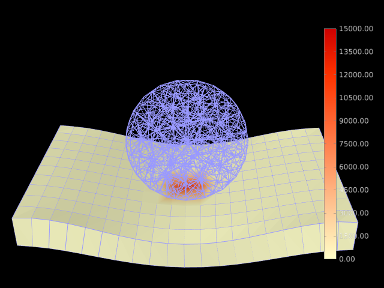
\includegraphics[]{images/ContactPressureRender}
\else
 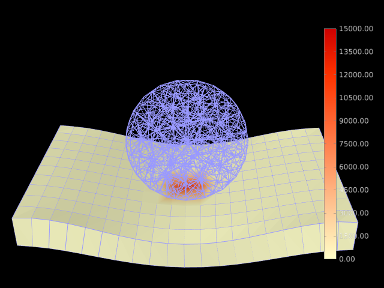
\includegraphics[width=3.75in]{images/ContactPressureRender}
\fi
\end{center}
\caption{ContactPressureRender showing the contact pressure as a
spherical FEM model falls onto an FEM sheet.  The color map is drawn
on the sheet model, with redder values indicating greater pressure.}
\label{ContactPressureRender:fig}
\end{figure}

The complete source code is shown below:
%
\lstset{numbers=left}
\lstinputlisting{../../src/artisynth/demos/tutorial/ContactPressureRender.java}
\lstset{numbers=none} 

To begin, the demo creates two FEM models: a spherical ball (lines
52-56) and a rectangular sheet (lines 59-66), and then fixes the end
nodes of the sheet (lines 69-74). Surface rendering is enabled for
the sheet (line 65), but not for the ball, in order to improve the
visibility of the color map.

Lines 77-81 create and set a collision behavior between the two
models, with the {\sf drawColorMap} property set to {\tt
CONTACT\_PRESSURE}. Because for this example we want the color map to
be drawn on the {\it second} collidable (the sheet), we set the {\sf
setColorMapCollidable} property to 1 (line 79); otherwise, the default
value of 0 would cause the color map to be drawn on the first
collidable (the ball). (Alternatively, we could have simply defined
the collision behavior as being between the surface and the ball
instead of the ball and the sheet.) The color map range is explicitly
set to lie between $[0, 15000]$ (line 80); this is in contrast to the
example in Section \ref{renderingDepth:sec}, where the range is
auto-updated on each step. The color range is also set explicitly in
the behavior, but if multiple objects were colliding it would likely
be preferable to set it in the collision manager (with the behavior's
value left as {\tt null}) to ensure a uniform render range across all
collisions.  Other rendering properties are set for the collision
manager at lines 83-97, including a custom color map that varies
between {\tt CREAM} (the color of the mesh) for no pressure and dark
red for maximum pressure.

At line 100, a color bar is created and added to the scene, using the
method {\tt createColorBar()} (lines 36-45), to explicitly show the
pressure that corresponds to the different colors. The color bar is
given the same color map and value range used to render the
pressure. Finally, default face and line colors for all components in
the model are set at lines 105-106.

To run this example in ArtiSynth, select {\sf All demos > tutorial >
ContactPressureRender} from the {\sf Models} menu. When run, the FEM
models will collide and render the contact pressure on the sheet, as
shown in Figure \ref{ContactPressureRender:fig}.

\ifdefined\maindoc
\else
\end{document}
\fi
